\documentclass[reqno]{amsart}
\usepackage[utf8]{inputenc}
\usepackage[margin=1in]{geometry}
\usepackage[usenames, dvipsnames]{xcolor}
\usepackage{graphicx}
\usepackage{mathtools}
\usepackage{amssymb}
\usepackage{amsthm}
\usepackage{fancyhdr}
\usepackage{adforn}
\usepackage{xparse}
\usepackage{tikz}
\usetikzlibrary{fadings}
%\usetikzlibrary{matrix, positioning, calc}
% Additional math macros that I want in both my notes and my psets
\usepackage[sc, noBBpl]{mathpazo}
\usepackage{mathrsfs}
\usepackage[T1]{fontenc}
\usepackage{calligra}
\usepackage{microtype}
\usepackage[all]{xy}
\usepackage{slashed}
\newcommand{\A}{\mathbb A}
\newcommand{\cat}{\mathsf}
\newcommand{\sC}{\cat C}
\newcommand{\sD}{\cat D}
\newcommand{\sS}{\cat S}
\newcommand{\sA}{\mathscr A}
\newcommand{\sF}{\mathscr F}
\newcommand{\sG}{\mathscr G}
\renewcommand{\P}{\mathbb P}
\newcommand{\cO}{\mathscr O}
\newcommand{\sI}{\mathscr I}
\DeclareMathOperator{\coker}{coker}
\renewcommand{\Im}{\operatorname{Im}}
\newcommand{\pt}{\mathrm{pt}}
\DeclareMathOperator{\Hom}{Hom}
\newcommand{\op}{^{\mathsf{op}}}
\newcommand{\Id}{\mathrm{Id}}
\DeclareMathOperator{\Mat}{Mat}
\newcommand{\m}{\mathfrak m}
%\newcommand{\p}{\mathfrak p}
\newcommand{\q}{\mathfrak q}
\DeclareMathOperator{\MSpec}{MSpec}
\DeclareMathOperator{\Spec}{Spec}
\newcommand{\Top}{\cat{Top}}
\newcommand{\Ring}{\cat{Ring}}
\newcommand{\Mod}{\cat{Mod}}
\DeclareMathOperator{\res}{res}
\newcommand{\Alg}{\cat{Alg}}
\newcommand{\Fun}{\cat{Fun}}
\newcommand{\AffSch}{\cat{AffSch}}
\newcommand{\Ab}{\cat{Ab}}
\DeclareMathOperator{\bl}{--}
\DeclareMathOperator{\Free}{Free}
\DeclareMathOperator{\For}{For}
\newcommand{\Set}{\cat{Set}}
\newcommand{\LocRing}{\cat{LocRing}}
\newcommand{\Grp}{\cat{Grp}}
\newcommand{\Sch}{\cat{Sch}}
\newcommand{\inHom}{\operatorname{\underline{\Hom}}}
\DeclareMathOperator{\Frac}{Frac}
\DeclareMathOperator{\Gal}{Gal}
\DeclareMathOperator{\Nil}{Nil}
\newcommand{\pre}{\sC^{\text{pre}}}
\newcommand{\sh}{_{\text{sh}}}
\newcommand{\G}{\mathbb G}
\DeclareMathOperator{\Proj}{Proj}
\newcommand{\sM}{\mathscr M}
\newcommand{\sV}{\mathscr V}
\newcommand{\fU}{\mathfrak U}
\newcommand{\GL}{\mathrm{GL}}
\DeclareMathOperator{\Sym}{Sym}
% http://tex.stackexchange.com/questions/141434/how-to-type-sheaf-hom
\DeclareMathOperator{\shom}{\mathscr{H}\text{\kern -4pt {\calligra\large om}}\,}
\newcommand{\sL}{\mathscr L}
\DeclareMathOperator{\QC}{QC}
\DeclareMathOperator{\Supp}{Supp}
\newcommand{\sN}{\mathscr N}
\DeclareMathOperator{\Ann}{Ann}
\DeclareMathOperator{\Der}{Der}
\newcommand{\ctcpx}[1]{(#1)^{\text{der}}}
\newcommand{\Dist}{\mathsf{Dist}}
\newcommand{\shdi}{\operatorname{Sh}_{\Dist}}
\DeclareMathOperator{\Sh}{Sh}
\newcommand{\shz}{\mathsf{Sh}_{\text{\rm Zar}}}
\DeclareMathOperator{\Gr}{Gr}
% Source: http://tug.org/pipermail/xy-pic/2001-July/000015.html
\newcommand{\pullbackcorner}[1][dr]{\save*!/#1+1.2pc/#1:(1,-1)@^{|-}\restore}
\newcommand{\pushoutcorner}[1][dr]{\save*!/#1-1.2pc/#1:(-1,1)@^{|-}\restore}
\newcommand{\TDel}{\mathrm{2\Delta}}
\DeclareMathOperator{\Bl}{B\ell}
\newcommand{\cR}{\mathcal R}
\newcommand{\cL}{\mathcal L}
\newcommand{\cH}{\mathcal H}
\newcommand{\refR}{\reflectbox{\(\cR\)}}

\renewcommand{\a}{\alpha}
\renewcommand{\b}{\beta}
%\newcommand{\e}{\epsilon}
\renewcommand{\l}{\lambda}
\renewcommand{\L}{\Lambda}
\newcommand{\g}{\gamma}
\newcommand{\s}{\sigma}
\newcommand{\z}{\zeta}
\newcommand{\RR}{\mathbb{R}}
\newcommand{\NN}{\mathbb{N}}
\newcommand{\QQ}{\mathbb{Q}}
\newcommand{\ZZ}{\mathbb{Z}}
\newcommand{\CC}{\mathbb{C}}
\newcommand{\cC}{\mathcal{C}}
\newcommand{\f}{\frac}
\newcommand{\p}{\partial}
\renewcommand{\P}[3][]{\f{\partial^{#1} #2}{\partial #3 ^{#1}}}
%\newcommand{\avg}[1]{\langle #1 \rangle}
\newcommand{\avg}[1]{\left< #1 \right>}
\newcommand{\?}{\overset{?}{=}}
\newcommand{\Int}{\int_{-\infty}^\infty}
\newcommand{\ket}[1]{\left| #1 \right>} % for Dirac bras
\newcommand{\bra}[1]{\left< #1 \right|} % for Dirac kets
\newcommand{\braket}[2]{\left< #1 \vphantom{#2} \right|
 \left. #2 \vphantom{#1} \right>} % for Dirac brackets
\newcommand{\pv}{\vec{p}}

\newcommand{\grad}[1]{\gv{\nabla} #1} % for gradient
\let\divsymb=\div % rename builtin command \div to \divsymb
\renewcommand{\div}[1]{\gv{\nabla} \cdot #1} % for divergence
\newcommand{\curl}[1]{\gv{\nabla} \times #1} % for curl
\renewcommand{\labelenumi}{(\alph{enumi})}
\let\vaccent=\v % rename builtin command \v{} to \vaccent{}
\renewcommand{\v}[1]{\ensuremath{\mathbf{#1}}}
\newcommand{\uv}[1]{\ensuremath{\mathbf{\hat{#1}}}} % for unit vector
\newcommand{\gv}[1]{\ensuremath{\mbox{\boldmath$ #1 $}}} 
% for vectors of Greek letters
\usepackage{hyperref}
\usepackage{siunitx}

%\usepackage[compat=1.1.0]{tikz-feynman}

% TODO fiddle with colors
\definecolor{newblue}{HTML}{1F98A6}
\definecolor{newred}{HTML}{D95448}
\definecolor{neworange}{HTML}{F29441}
\hypersetup{
	colorlinks,
	linkcolor=newred,
	citecolor=neworange,
	urlcolor=newblue!80!black,
}
\usepackage[all]{hypcap}
\pagestyle{plain}
\setcounter{tocdepth}{1}


\usepackage{titlesec}
\titleformat{\section}[frame]
  {\normalfont}
  {\filright
   \footnotesize
   \enspace Lecture \arabic{section}.\enspace}
  {8pt}
  {\Large\bfseries\filcenter}
\usepackage[dotinlabels]{titletoc}
\titlecontents{section}[1.5em]{}{\contentslabel{2.3em}}{\hspace*{-2.3em}}{\hfill\contentspage}

\renewcommand{\sectionmark}[1]{\markleft\thesection. #1}

\fancyhf{}
\fancyhead[RO,LE]{\small\thepage}
\fancyhead[LO]{\small\slshape\nouppercase{\rightmark}}
\fancyhead[RE]{\small\slshape Advanced Quantum Field Theory Lecture Notes}
\setlength{\headheight}{11.0pt}
\pagestyle{fancy}

\numberwithin{equation}{section}
\newcommand{\orbreak}{
\begin{center}
	\adforn{17}\;\(\cdot\)\;\adforn{18}
	\vspace{0.2cm}
\end{center}
}

\renewcommand{\labelitemi}{\(\circ\)}

% I wanted to allow one to reference parts of a thm/cor/etc. and have it print the thm number too, e.g. 29.2(1),
% but this isn't working right now. Probably the best way to do this would be to play around with enumitem to
% define a new enumerate-like counter and then just use that directly instead of enumerate in comp.

% This feels really wobbly, but so far it's working
\NewDocumentEnvironment{comp}{mm}{%
	\csname #1\endcsname\hfill
	\csname #2\endcsname
}{
	\csname end#2\endcsname
	\csname end#1\endcsname
}

% usage:
% \shortexact[f][g]{A}{B}{C},
%
%			 f    g
% for 0 -> A -> B -> C -> 0,
\DeclareDocumentCommand{\shortexact}{O{} O{} mmmm}{
\xymatrix{
	0\ar[r] & #3\ar[r]^-{#1} & #4\ar[r]^-{#2} & #5\ar[r] & 0#6
}}
% exactly the same, but for 0 -> A -> B -> C
\DeclareDocumentCommand{\leftexact}{O{} O{} mmmm}{
\xymatrix{
	0\ar[r] & #3\ar[r]^-{#1} & #4\ar[r]^-{#2} & #5 #6
}}
% ... and the same, for A -> B -> C -> 0
\DeclareDocumentCommand{\rightexact}{O{} O{} mmmm}{
\xymatrix{
	#3\ar[r]^-{#1} & #4\ar[r]^-{#2} & #5\ar[r] & 0#6
}}



% usage:
% X\dblarrow[r] & Y
%   f
% X => Y
%   g
\DeclareDocumentCommand{\dblarrow}{O{} O{} O{}}{
	\ar@<0.4ex>[#1]^-{#2}\ar@<-0.4ex>[#1]_-{#3}
}
% Note: it would be a useful exercise to figure out how to define this so it can be used as
% \dblarrow[r]^f_g

\everyentry={\displaystyle}

\newcommand{\N}{\mathbb N}
\newcommand{\Z}{\mathbb Z}
\newcommand{\Q}{\mathbb Q}
\newcommand{\R}{\mathbb R}
\newcommand{\C}{\mathbb C}
\newcommand{\F}{\mathbb F}
\newcommand{\vp}{\varphi}
\newcommand{\term}{\emph}
\renewcommand{\vec}[1]{\boldsymbol{\mathbf{#1}}}
\DeclarePairedDelimiter\paren{(}{)}
%\DeclarePairedDelimiter\ang{\langle}{\rangle}
\DeclarePairedDelimiter\abs{\lvert}{\rvert}
\DeclarePairedDelimiter\norm{\lVert}{\rVert}
\DeclarePairedDelimiter\bkt{[}{]}
\DeclarePairedDelimiter\set{\{}{\}}
% Swap paren* and paren, etc., so that the normal version resizes by default.
% Meanwhile, one can use \paren*[\Big]{...} to customize the size easily.
% It would be interesting to wrap this up into a custom \definedelimiter command...
\makeatletter
	\let\oldparen\paren
	\def\paren{\@ifstar{\oldparen}{\oldparen*}}
	\let\oldbkt\bkt
	\def\bkt{\@ifstar{\oldbkt}{\oldbkt*}}
\makeatother
\newcommand{\e}{\varepsilon}
\def\qedsymbol{{\small{\ensuremath{\boxtimes}}}}
\newcommand{\inj}{\hookrightarrow}
\newcommand{\surj}{\twoheadrightarrow}
\DeclareMathOperator{\id}{id}
\newcommand{\ud}{\,\mathrm{d}}
\renewcommand{\d}{\mathrm d}
\newcommand{\dfr}[2]{\frac{\mathrm d #1}{\mathrm d #2}}
\newcommand{\pfr}[2]{\frac{\partial #1}{\partial #2}}

%\catcode`\"=13
%\newcommand{"}[1]{^{(#1)}}
\newtheorem{thm}[equation]{Theorem}
\newtheorem*{thm*}{Theorem}
\newtheorem{lem}[equation]{Lemma}
\newtheorem*{lem*}{Lemma}
\newtheorem{cor}[equation]{Corollary}
\newtheorem{prop}[equation]{Proposition}
\newtheorem{obs}[equation]{Observation}
\theoremstyle{definition}
\newtheorem{ex}[equation]{Exercise}
\newtheorem{exm}[equation]{Example}
\newtheorem{defn}[equation]{Definition}
\newtheorem*{claim}{Claim}
\theoremstyle{remark}
\newtheorem*{rem}{Remark}
\newtheorem*{fct}{Fact}
\newtheorem*{note}{Note}

\begin{document}
\title{String Theory}
\author{Ian Lim\\ Last updated \today}
\maketitle
{\small\noindent These notes were taken for the \textit{String Theory} course taught by R.A. Reid-Edwards at the University of Cambridge as part of the Mathematical Tripos Part III in Lent Term 2019. I live-\TeX ed them using Overleaf, and as such there may be typos; please send questions, comments, complaints, and corrections to 
\href{mailto:itel2@cam.ac.uk?subject=STR\%20Lecture\%20Notes}{\texttt{itel2@cam.ac.uk}}.\\
Many thanks to Arun Debray for the {\LaTeX} template for these lecture notes: as of the time of writing, you can find him at \url{https://web.ma.utexas.edu/users/a.debray/}.}

\tableofcontents

\section{Friday, January 18, 2019}
	\begin{note}
    Here's the relevant admin content for the first day. The lecturer's email is \url{n.datta@damtp.cam.ac.uk}., and course notes can be found on the CQIF webiste under Part III lectures.
\end{note}

Quantum information theory (QIT) was born out of classical information theory (CIT).
\begin{defn}
Classical information theory is the mathematical theory of information processing tasks, e.g. storage, transmission, processing of information.
\end{defn}
In contrast, quantum information theory asks how these tasks can be performed if we harness quantum mechanical systems as information carriers. Such systems include electrons, photons, ions, etc.

QM has some novel features which are not present in our old Newtonian theories. We know that quantum systems obey the Heisenberg uncertainty principle, that energy is quantized in these systems, and QM systems cannot generically be copied (the famous no-cloning theorem).
Quantum mechanically, one can describe the full state of a system without knowing the state of the subsystems-- this is essentially the idea of entanglement.%
    \footnote{If you like, some composite states in a tensor product space cannot be decomposed into a direct product.}

Here's a quick overview now of the structure of the course.
\begin{itemize}
    \item Basic concepts of CIT
    \item Study of open quantum systems
    \item Mathematical tools for QIT
    \item Entanglement
    \item QIT itself
\end{itemize}
When we say open quantum systems, we mean quantum systems which interact with a broader environment. If we prepare a state and allow it to interact, what happens to the information stored in that state?

\subsection*{Classical information theory} Historically, CIT was invented in 1948 with a pioneering paper by Claude Shannon. In this paper, he asked two critical questions.
\begin{itemize}
    \item[Q1.] What is the limit to which information can be \emph{reliably} compressed?
    \item[Q2.] What is the maximum rate at which information can be reliably sent through a communication channel?
\end{itemize}
That is, we may ask about how to encode information in such a way that it can still be recovered with a high probability of success. And we can ask how to send this information when our communication channels will naturally be noisy. The answers to these questions are known as \term{Shannon's Source Coding Theorem} and \term{Shannon's Noisy Channel Coding Theorem}, respectively.

\subsection*{What is information?} We have an intuitive sense of what information means, but to formalize this takes a little work. In the loosest sense, information is associated to uncertainty and in particular information gain is related to a reduction in uncertainty.
\begin{exm}
Suppose I have a system which takes some discrete values, e.g. I roll a fair die. The outcome is a variable $x$ which takes values in some set, $J=\set{1,2,\ldots, 6}$. We write that capital $X$ is proportional to $p(x),x\in J$, where $P(X=x)=p(x)=1/6\, \forall x\in J$. That is, there is a probability mass function associated to the possible outcomes. The probability that we measure the system $X$ in outcome $x$ is $1/6$ for any outcome $x$ in the set of outcomes.
\end{exm}

We also define the following quantity.
\begin{defn}
\term{Surprisal} is the quantity
\begin{equation}
    \gamma(x)=-\log p(x).
\end{equation}
When an event is very unlikely and it happens anyway... you are very surprised. For example, $p(x)=1\implies \gamma(x)=0$ (certainties are not very surprising) while $p(x)\approx 0 \implies \gamma(x)$ large.
\end{defn}
This quantity has some features:
\begin{itemize}
    \item It only depends on $p(x)$ and not on $x$.
    \item It is a continuous function of $p(x).$
    \item It is additive for independent events.
\end{itemize}
This last property is easy to prove:
\begin{equation*}
    P(X=x,Y=y)=P_{XY}(x,y)=P_X(x)P_Y(y)
\end{equation*}
when $X,Y$ are independent. Then
\begin{equation*}
    \gamma(x,y)=-\log P_{XY}(x,y)=\gamma(x)+\gamma(y).
\end{equation*}

\begin{defn}
    We can now define the \term{Shannon entropy} of $X$ to be
    \begin{equation}
        H(X)\equiv \mathbb{E}(\gamma(X))=\sum_{x\in J}(-\log(p(x))p(x),
    \end{equation}
    the expected value of the surprisal. We see again that $H(X)$ does not depend on the actual outcomes themselves but only on the probability distribution $P(X)$.
\end{defn}
As a matter of convention we will take logs to be $\log{} \equiv \log_2{}$, and for events which are impossible $P(x)=0$ we have $0\log 0 = 0$ (which one can prove by taking the limit $\lim_{u\to 0}u\log u =0.$

\subsection*{Binary entropy} Consider an event which has two possible outcomes, $X\sim P(x), x\in J =\set{0,1}$ where $P(X=0)=p$ and $P(X=1)=1-p$. Then the Shannon entropy is
\begin{equation}
    H(X)=-p\log p - (1-p)\log(1-p)\equiv h(p).
\end{equation}
We see that if the probability is $p=1/2$, then we have no information a priori about this systems-- the entropy is maximized. $h(p)$ is a continuous function of $P$, and it is concave.

\begin{defn}
    We can also define a different entropy, the Renyi entropy, which is
    \begin{equation}
        H_\alpha(X)=\frac{1-\alpha}\log (\sum_{x\in J}P(x)^\alpha),
    \end{equation}
    with $\alpha \in (1,2]$. As an exercise, we can verify that $\lim_{\alpha \to 1} H_\alpha(X) = H(X)$, i.e. the Renyi entropy reduces to the Shannon entropy.
\end{defn}

Why do we choose to work with the Shannon entropy? It has to do with the operational interpretation-- the Shannon entropy represents an optimal rate of data compression, i.e. the data compression limit.

In CIT, a classical information source emits some messages/data/signals/information. For instance, $J$ could output a binary output or perhaps telegraph English (26 letters and a space). Now, the simplest class of sources is \term{memoryless}-- they are ``independent identically distributed'' sources (i.i.d.), which means that successive messages are independent of each other, and they are identically distributed.

\begin{defn}
    Suppose we have some random variables $U_1,U_2,\ldots, U_n$ with $U_i \sim p(u),u\in J$. We say these are \term{identically distributed} if
    \begin{equation*}
        p(u)=P(U_k=u), u\in J \quad \forall 1\leq k \leq n.
    \end{equation*}
\end{defn}
We could study a signal emitted by $n$ uses of the source to get some sequence $\underline{u}^{(n)}=(u_1,u_2,\ldots, u_n)$.
\begin{defn}
    Moreover, if the probability mass function takes the form
    \begin{align*}
        p(\underline{u^{(n)}}) &=P(U_1,\ldots,U_n= u_n)\\
        &= p(u_1)\ldots p(u_n).
    \end{align*}
\end{defn}

If the source is indeed independent and identically distributed, then it makes sense to describe it by a sincle probability mass function, $U\sim p(u)$, so that the Shannon entropy of the source can be siad to be
\begin{equation}
    H(U)=-\sum_{u\in J} p(u) \log p(u).
\end{equation}

Another guiding question. Why is data compression possible? Our information source has some \emph{redundancy}. For instance, in the English language, certain letters are more common than others, so we can encode something that is more common in a shorter string in anticipation it will be used more often.

This sort of scheme is known as variable length coding, e.g. we might encode the letter ``e'' as the string $10$ and the letter ``z'' as $11000$. In contrast, we could also use a fixed length coding scheme where we have a ``typical set'', a subset of our total outcomes $J^n$ (things we might like to encode). Our typical set then has a one-to-one mapping to the set of encoded messages, e.g. $\set{0,1}^m$, so we can always recover them precisely, while several outcomes outside the typical set might map to the same encoded message. There's some probability that we'll want to encode things outside the typical set, and in decoding we'll get the original message a little bit wrong. But if we choose the typical set well, this can be made to be a rare occurrence. We are usually interested in \emph{asymptotic i.i.d.} settings, i.e. in the limit as the size of the set of possible messages to be encoded goes to $\infty$.

\begin{exm}
    Suppose we have a horse race with eight horses. They have labels $1,2\ldots, 8$, and the message we would like to encode is the label of the winning horse. A priori, we only need $3$ bits to encode the label since $2^n$ different messages can be stored in $n$ bits.
    
    However, what if the horses are of different abilities? Realistically, they won't all be equally fast. Suppose that $p_i$ is the probability of the $i$th horse winning, such that
    \begin{equation*}
        p_i=1/2,1/4,1/8,1/16,1/64,\ldots,1/64.
    \end{equation*}
    Now we assign the following code words:
    \begin{align*}
        C(1)&=0\\
        C(2)&=10\\
        C(3)&=110\\
        C(4)&=1110\\
        C(5)&=111100\\
        C(6)&=111101\\
        \vdots&
    \end{align*}
    Let $l_i$ be the length of the $i$th codeword, e.g. $l_5=6$. We can show that the average length of a code is then $\sum p_i l_i = 2$, and we've chosen a prefix-free code so that e.g. a sequence like 10011001110 can be uniquely decoded to a sequence of winners from our code words.
\end{exm}

\section{Monday, January 21, 2019}
    Last time, we introduced a \term{worldline action} with an einbein $e$ (auxiliary field).
\begin{equation*}
    S[x,e]=\frac{1}{2}\int d\tau \left(e^{-1} \eta_{\mu\nu} \dot x^\mu \dot x^\nu-e m^2\right).
\end{equation*}
In the massless limit, this reduces to
\begin{equation}
    S[X,e]=\frac{1}{2} d\tau e^{-1} g_{\mu\nu} \dot x^\mu \dot x^\nu,
\end{equation}
where we have replaced the Minkowski metric with some generic metric. The classical equations of motion for $X^\mu(\tau)$ then give the geodesic equation,
\begin{equation}
    \ddot X^\mu +\Gamma^\mu_{\nu\lambda} \dot X^\nu \dot X^\lambda = 0.
\end{equation}
The $e(\tau)$ equations of motion would give some constraints. However, if we attempted to quantize this theory, we would find that the background metric $g_{\mu\nu}$ is not actually deformed in the solutions. Rather than being dynamic as in general relativity, it's sort of a thing that is given to us and sits in the background, unchanging, which is why for a particle this is not a theory of quantum gravity. As we'll see, this is \emph{not} the case for strings.

\subsection*{Strings} As a string moves through some flat spacetime $\cM$ with metric $\eta_{\mu\nu}$, it sweeps out a worldsheet $\Sigma.$ Assume that the string is closed, so it has a coordinate $\sigma$ (along the length of the string, if you like):
\begin{equation*}
    \sigma \sim \sigma + 2n\pi, n\in \ZZ.
\end{equation*}
And it moves through time as parametrized by a proper time $\tau$, so the embedding of the worldsheet is given by $X^\mu(\sigma,\tau)$. That is, $\sigma$ and $\tau$ provide good coordinates for the worldsheet in $\cM$.
\begin{defn}
    We call these $X^\mu$ embedding fields. They are maps
    $X:\Sigma \to \cM$ from the worldsheet to the background spacetime manifold.
\end{defn}
We also say that the area of the worldsheet $\Sigma$ is given by
\begin{equation}
    \text{area}=\int d\tau d\sigma \sqrt{-\det(\eta_{\mu\nu} \p_a X^\mu \p_0 X^\nu)}
\end{equation}
where $\sigma^a =(\tau, \sigma)$ so that $\p_a = \P{}{\sigma^a}.$ In fact, we shall introduce an extra factor know (for historical reasons) as $\alpha'$ and write
\begin{equation}\label{nambugoto}
    S[X]=-\frac{1}{2\pi \alpha'}\int d\tau d\sigma \sqrt{-\det(\eta_{\mu\nu} \p_a X^\mu \p_b X^\nu)},
\end{equation}
where $\alpha'$ is a free parameter. We often refer to the \term{string length},
\begin{equation}
    l_s \equiv 2\pi\sqrt{\alpha'}
\end{equation}
or the \term{tension}
\begin{equation}
    T \equiv \frac{1}{2\pi \alpha'}.
\end{equation}

\begin{defn}
    The object
    \begin{equation}
        G_{ab}\equiv \eta_{\mu\nu} \p_a X^\mu \p_b X^\nu
    \end{equation}
    is an induced metric on $\Sigma$, and the action \ref{nambugoto} is called the \term{Nambu-Goto action}.
\end{defn}
Having just defined this, we won't really do anything with it for the rest of the course. Bummer. However, to make up for it, let's write down a new and improved action, the \term{Polyakov action}.

\begin{defn}
    Consider the action
    \begin{equation}\label{polyakovaction}
        S[X,h]=-\frac{1}{4\pi \alpha'} \int_\Sigma d^2\sigma \sqrt{-h}\,h^{ab} \eta_{\mu\nu} \p_a X^\mu \p_b X^\nu.
    \end{equation}
    This should remind us of what we did with the einbein last lecture, where we introduced $e$ into our action.
    
    This \term{Polyakov action} is classically equivalent to the Nambu-Goto action, since this auxiliary $h$ which we have introduced will turn out to be non-dynamical.
\end{defn}

The $h_{ab}$ equations of motion are given by a weird variation of the action,
\begin{equation}
    -\frac{2\pi}{\sqrt{-h}}\frac{\delta S}{\delta h^{ab}}=0.
\end{equation}
These equations of motion give the vanishing of the stress tensor, $T_{ab}=0$, where
\begin{equation}
    T_{ab}=-\frac{1}{\alpha'}\paren{\p_a X^\mu \p_b X_\mu - \frac{1}{2} h_{ab} \p_c X^\mu \p_d X_\mu h^{cd}}.
\end{equation}

Note that in two dimensions, $T_{ab}h^{ab}=0$, i.e. $T_{ab}$ is traceless. This is our first indication that something is different about two dimensions.

The $X^\mu$ equations of motion are
\begin{equation}
    \frac{1}{\sqrt{-h}}(\p_a \sqrt{-h}\, h^{ab} \p_b X^\mu)=0, \quad
    \Box X^\mu =0.
\end{equation}
Now we could imagine adding a cosmological constant (which would cause the trace of the stress tensor to change) or perhaps some sort of Einstein-Hilbert term to our metric $h_{ab}$. But we'll see why this might be more complicated than it initially seems.

\subsection*{Symmetries} The Polyakov action \ref{polyakovaction} has the following symmetries:
\begin{itemize}
    \item Rigid (global) symmetry, $X^\mu(\sigma,\tau)\to \Lambda^\mu{}_\nu X^\nu(\sigma,\tau) + a^\mu$ (Poincar\'e invariance).
    \item Local symmetries-- the physics should be invariant under reparametrizations of the coordinates of the worldsheet, so under transformations $\sigma^a \to \sigma'{}^a (\sigma,\tau).$ The fields themselves transform as
    \begin{align*}
        X'^\mu(\sigma',\tau')&= X^\mu(\sigma,\tau)\\
        h_{ab}(\sigma,\tau)&= \P{\sigma'{}^c}{\sigma^a} \P{\sigma'{}^d}{\sigma^b} h'_{cd}(\sigma',\tau').
    \end{align*}
    Infinitesimallly, this means that $\sigma^a \to \sigma^a - \xi^a(\sigma,\tau)$, which gives us the variations
    \begin{align*}
        \delta X^\mu &= \xi^a \p_a X^\mu\\
        \delta h_{ab} &= \xi^c \p_c h_{ab}+\p_a \xi^c h_{cb} +\p_b \xi^c h_{ca} =\nabla_a \xi_b +\nabla_b \xi_a\\
        \delta \sqrt{-h} &=\p_a(\xi^a \sqrt{-h}).
    \end{align*}
    Note this second variation, $\delta h_{ab}$, can be written in terms of some covariant derivatives for an appropriate connection, but we won't usually bother.
    \item Weyl transformations-- we send
    \begin{align*}
        X'{}^\mu (\sigma,\tau) &= X^\mu(\sigma, \tau)\\
        h'_{ab}(\sigma,\tau)&=e^{2\Lambda(\sigma,\tau)}h_{ab}(\sigma,\tau).
    \end{align*}
    Thus $\delta X^\mu=0$ and $\delta h_{ab}=2\Lambda h_{ab}$.
    Under such transformations, we have three arbitrary degrees of freedom in $(\xi^a,\Lambda)$ (two from the two components of $\xi$ plus one from $\Lambda$), and we can use them to fix the three degrees of freedom in $h_{ab}$ (there are three, since $h$ is symmetric and $2\times 2$).
\end{itemize}

\subsection*{Classical solutions} Let us now use reparametrization invariance to fix
\begin{equation}
    h_{ab}=e^{2\phi} \eta_{ab}, \quad \eta_{ab}=\begin{pmatrix}
    -1 & 0\\
    0 & 1
    \end{pmatrix}.
\end{equation}
The Polyakov action then becomes
\begin{equation}
    S[X]=-\frac{1}{4\pi \alpha'} \int_\Sigma d^2 \sigma(-\dot X^2 + X'{}^2),
\end{equation}
where
\begin{equation}
    \dot X^\mu \equiv \P{X^\mu}{\tau},\quad X'{}^\mu \equiv \P{X^\mu}{\sigma}
\end{equation}
and squares are taken by contracting with the metric $h_{ab}$. In that case, the $X^\mu(\sigma,\tau)$ equation of motion becomes the wave equation in 2D, %check this?
so solutions are of the form
\begin{equation}
    X^\mu(\sigma,\tau)= X^\mu_R (\tau-\sigma)+X^\mu_L(\tau + \sigma).
\end{equation}
Moreover, since we have a wave equation it is useful to introduce modes $(\alpha^\mu_n, \bar \alpha^\mu_n)$ where
\begin{equation}
    X^\mu_R(\tau-\sigma)=\frac{1}{2}x^\mu +\frac{\alpha'}{2}p^\mu(\tau-\sigma) +i\sqrt{\frac{\alpha'}{2}}\sum_{n\neq 0} \frac{1}{n}
    \alpha^\mu_n e^{-in(\tau-\sigma)},
\end{equation}
where $x^\mu, p^\mu$ are some constants in $(\tau,\sigma)$ and  similarly the left-going modes are
\begin{equation}
    X^\mu_L(\tau+\sigma)=\frac{1}{2}x^\mu +\frac{\alpha'}{2}p^\mu(\tau+\sigma) +i\sqrt{\frac{\alpha'}{2}}\sum_{n\neq 0} \frac{1}{n}
    \bar\alpha^\mu_n e^{-in(\tau+\sigma)}.
\end{equation}
It's sometimes useful to define a zero-mode,
\begin{equation}
    \alpha_0^\mu = \bar \alpha_0^\mu = \sqrt{\frac{\alpha'}{2}}p^\mu.
\end{equation}

\section{Wednesday, January 23, 2019}
    Let's recall the statement of Shannon's source coding theorem. Shannon tells us that if we have an iid source $U\sim p(u); u\in J$ with Shannon entropy $H(U)$, then there is a fundamental limit on data compression given by $H(U)$ such that for any rate $R>H(U)$, there exists a reliable compression-decompression scheme of rate $R,$ and conversely for any rate $R<H(U)$, any scheme of rate $R$ will not be reliable.

See my notes from last lecture for a heuristic argument of the converse. The formal argument can be made with $\epsilon$s and $\delta$s-- for example, my statement that we need not consider elements in $A_\epsilon^{(n)}$ is equivalent to $\sum_{\underline{u}^{(n)}\in S^n \cap A_\epsilon^n} p(\underline{u}^{(n)}) \leq P(A_\epsilon^n \to 0$.

\subsection*{Entropies} Consider a pair of random variables $X,Y$ with \term{joint probability}
\begin{equation}
    P(X=x,Y=y)=P_{XY}(x,y)=p(x,y).
\end{equation}
Here, $x\in J_X$ some alphabet and similarly $y\in J_Y$. We can also define the conditional probability
\begin{equation}
    P(Y=y|X=x)=p(y|x),
\end{equation}
the probability of $y$ given $x$.

\begin{defn}
    Now we have the \term{joint entropy}, which is
    \begin{equation}
        H(X,Y)\equiv -\sum_{x\in J_X,y\in J_Y} p(x,y)\log p(x,y).
    \end{equation}
\end{defn}
\begin{defn}
    We also have the \term{conditional entropy}, which is
    \begin{align*}
        H(Y|X) &\equiv \sum_x p(x) H(Y|X=x)\\
        &= -\sum_x p(x) \sum_y p(y|x) \log p(y|x).
    \end{align*}
\end{defn}
But we can simplify this to write
\begin{equation}
    H(Y|X)=-\sum p(x,y) \log p(y|x),
\end{equation}
which implies that
\begin{equation}
    p(x,y)= p(x) p(y|x) = p(y)p(x|y).
\end{equation}
This leads us to a chain rule,
\begin{equation}
    H(X,Y)= H(Y|X) + H(X).
\end{equation}

We also have the notion of a relative entropy, which measures a ``distance'' between two probability distributions. Suppose we have distributions $p=\set{p(x)}_{x\in J}$ and $q=\set{q(x)}_x\in J$, Let us assume that the $\text{supp}p \subseteq \text{supp} q$, with $\text{supp} p = \set{x\in J: p(x) >0}$. This implies that $q(x)=0\implies p(x)=0$, which we denote $p\ll q$.
\begin{defn}
    Thus we define the \term{relative entropy} to be
    \begin{equation}
        D(p||q)  \equiv \sum_{x\in J} p(x) \log \frac{p(x)}{q(x)}.
    \end{equation}
    If $p\ll q$, then this is well-defined (otherwise we might have $q\to 0$ with $p$ nonzero). Taking $0\log \frac{0}{q(x)}=0$ we see that this represents a sort of distance,
    \begin{equation}
        D(p||q) \geq 0
    \end{equation}
    with equality iff $p=q$.
\end{defn}
This is not quite a true metric, since it is not symmetric, $D(p||q)\neq D(q||p)$, and moreover it does not satisfy a triangle inequality, i.e. $D(p||r)\not\leq D(p||q) +D(q||r)$.

Using the relative entropy, we can now define a useful quantity known as the mutual information.
\begin{defn}
    The mutual information between two sources $X$ and $Y$ is
    \begin{align*}
        I(X;Y) &= H(X)+ H(Y) - H(X,Y)\\
        &= H(X)- H(X|Y).
    \end{align*}
\end{defn}
The mutual information has some intuitive properties.
\begin{itemize}
    \item $I(X:X)=H(X)$, since $I(X;X)=H(X)+H(X)-H(X,X)= H(X)$.
    \item $I(X;Y) = I(Y;X)$
    \item if $X,Y$ independent, then $I(X;Y)=0$.
\end{itemize}

Suppose now we have $P,Q$ taking non-negative real values, with $Q(x)=0 \implies P(X)=0$. THus the relative entropy is
\begin{equation*}
    D(P||Q)=\sum P(x) \log \frac{P(x)}{Q(x)}.
\end{equation*}
What if $P(x)=p(x), x\in J$ and $Q(x)=1 \forall x \in J$? Then
\begin{equation}
    D(P||Q)=\sum_x p(x) \log p(x) = -H(X).
\end{equation}
It's almost trivial to check that if $Q(x)=\frac{1}{|J|}$ instead, then we would get an additional factor of $-\log |J|.$

\begin{ex}
Check that the mutual information satisfies
\begin{equation}
    I(X;Y)=D(p(x,y)|| p(x) p(y)).
\end{equation}
\end{ex}

Let's take a minute to prove the non-negativity of the relative entropy. That is, $D(p||q) \geq 0$.
\begin{proof}
By definition,
\begin{equation}
    D(p||q) = \sum_{x\in J}p(x) \log\frac{p(x)}{q(x)}.
\end{equation}
Let us define a set $A$ such that
\begin{equation*}
    A=\set{x\in J \text{ s.t. } p(x) > )}.
\end{equation*}
Thus $A$ is the support of $J$.
We can compute
\begin{align}
    -D(p||q) &= \sum p(x) \log \frac{q(x)}{p(x)}\\
    &= \mathbb{E}_p \paren{\log \frac{q(X)}{p(X)}}.
\end{align}
Note that $X$s denote random variables, while $x$s indicate the values they take.

Jensen's inequality from probability theory tells us that for convave functions $f$, $\mathbb{E}(f(X)) \leq f(\mathbb{E}(X)).$

We conclude that 
\begin{align*}
    -D(p||Q)&\leq \log (\mathbb{E}_p \frac{q(X)}{p(X)})\\
    &= \log \sum_{x\in A} p(x) \frac{q(x)}{p(x)}\\
    &\leq \log \sum_x\in J q(x)\\
    &= \log 1 =0\\
    &\implies D(p||Q)\geq 0.
\end{align*}
\end{proof}

Suppose we had a distribution $p=\set{p(x)}, q(x)\frac{1}{|J|}\forall x\in J$ as before. Then
\begin{align}
    0\leq D(p||q) &= \sum p(x) \log \frac{p(x)}{(1/|J|)}\\
    &= -H(X)+ \sum p(x) \log |J|\\
    \implies H(X) &\leq \log|J|.
\end{align}
    
\section{Friday, January 25, 2019}
    Last time, we introduced many important classical concepts. We talked about the mutual (common) information $I(x:Y)$ between two sources, arguing that
\begin{align*}
    I(X:Y) &= H(X) + H(Y) - H(X,Y)\\
        &= H(X) - H(X|Y)\\
        &= H(Y)- H(Y|X).
\end{align*}
In particular we find that $I(X:X)=H(X), I(X:Y)=I(Y:X),$ and $I(X:Y)=0$ iff $X,Y$ are independent.

We can also prove that the mutual information is non-negative,
\begin{equation}
    I(X:Y) \geq 0,
\end{equation}
which follows from writing in terms of the conditional entropy as $H(X)-H(X|Y) \geq 0$. Equivalently we should show that
\begin{equation}
    H(X|Y) \leq H(X).
\end{equation}
That is, \emph{conditioning reduces entropy}.

We may describe the concavity of $H(X)$-- that is, for two sources with $X,Y; J$ with $\lambda\in [0,1]$
\begin{equation}
    H(\lambda p_X +(1-\lambda)p_Y) \geq \lambda H(p_x) + (1-\lambda) H(p_Y),
\end{equation}
which we will prove on the first examples sheet. This is analogous to what we showed in a few lines about the binary entropy.

The Shannon entropy of $H(X,Y)$ (where we simply replace $p(x)$s in the definition of $H(X)$ with $p(x,y)$) is constrained by the following inequality:
\begin{equation}
    H(X,Y) \geq H(X) + H(Y).
\end{equation}
This property is known as \term{subadditivity}.

We also have the property that the conditional entropy is non-negative--
\begin{equation}
    H(X|Y) \geq 0.
\end{equation}
Equivalently, $H(X,Y) - H(Y) \geq 0$
We shall see that once we introduce quantum correlations, this will no longer be true.

\subsection*{Data processing inequality}
Suppose we have some variables $X_1,X_2,\ldots$. In a Markov chain, we say that the probability of some outcome $X_n=x_n$ in a chain is
\begin{equation}
    P(X_n=x_n | X_1=x_1 \ldots X_{n-1} = x_{n-1}) = P(X_n = x_n | X_{n-1} = x_{n-1}).
\end{equation}
That is, the value of a Markov chain at a position $n$ depends only on its value at $n-1$.

Consider a simple Markov chain with three variables, $X\to Y \to Z$.
\begin{center}
    \begin{tikzpicture}[scale=2, node distance = 3.5cm, auto]
        \node [] (start) {};
        \node [block, right of=start] (noisy) {noisy channel};
        \node [block, right of=noisy, node distance=4cm] (process) {data processing};
        \node [right of=process] (end) {};
        
        \path [line] (start) -- node[above] {$X$} node[below] {input} (noisy);
        \path [line] (noisy) -- node[above] {$Y$} node[below] {output} (process);
        \path [line] (process) -- node[above] {$Z$} node[below] {processed} (end);
    \end{tikzpicture}
\end{center}
Then by the definition of a Markov chain, $P(Z=z| X=x, Y=y) = P(Z=z| Y=y)$, and we can prove that
\begin{equation}
    I(X:Z) \leq I(X:Y),
\end{equation}
known as the \term{data processing inequality} (DPI). That is, there is no data processing that can increase the correlation between two random variables.

\subsection*{Chain rules} Chain rules are relations between different entropy quantities, e.g. $H(X,Y)=H(X)+ H(Y|X)$. Suppose we have three random variables $X,Y,Z$ with a joint probability of $p(x,y,z)$.
\begin{ex}
    Prove that
    \begin{equation}
        H(X,Y,Z)=H(X) + H(Y|X) + H(Z|X,Y).
    \end{equation}
\end{ex}
\begin{defn}
    Now one can define the \term{conditional mutual information} as follows:
    \begin{equation}
        I(X:Y | Z) := H(X|Z) - H(X|Y,Z) \geq 0,
    \end{equation}
    with equality when $X-Y-Z$ forms a Markov chain.
\end{defn}

We have one more topic for classical information theory-- it is \term{Shannon's Noisy Channel Coding Theorem.} As usual, let us work in the asymptotic iid limit.

Suppose we have some source $X$ producing outputs in an alphabet $J_X$, and some received signals $Y\in J_Y$. We also have a noisy channel $\mathcal{N}:J_X \to J_Y$, and a stochastic map, defined to be a set of probabilities $\set{p(y|x)}$.

Here's the setup. Alice wants to send a message $m$ to her friend Bob. To do this, she takes her message $m\in \cM$ a set of messages and runs an encoding process $\mathcal{E}_n$ to produce a codeword $x^{(n)}_m$. She uses the (possibly noisy) channel $\mathcal{N}$ multiple times, say $n$ times, to send a transmitted message $y_m^{(n)}\neq x_m^{(n)}$, which Bob then runs a decoding process $\mathcal{D}_n$ on to get a final decoded message $m'$.

If $m'\neq m,$ we have gotten an error. In the $n\to \infty$ limit, we would like the probability of error $p_err^{(n)}=p(m'\neq m) \to 0$.

In some sense, encoding is like the dual process of compression. In encoding, we add redundancy in a controlled manner to account for the potential noise of the channel $\mathcal{N}$.

\begin{defn}
    We define a \term{discrete channel} to be the following:
    \begin{itemize}
        \item An input alphabet $J_X$
        \item An output alphabet $J_Y$
        \item A set of conditional probabilities (dependent on the number of uses $n$) $\set{p(\underline y^{n}| \underline x^{n})}$.
    \end{itemize}
\end{defn}
The input to $n$ uses of the channel sends $n$ uses of the source, $\underline{x}^{(n)}=(x_1,\ldots, x_n)\in J_X^n$ to an output $\underline{y}^{(n)}=(y_1\ldots y_n)\in J_Y^n$ with probability $p(\underline y^{n}| \underline x^{n})$.

We can consider memoryless channels, i.e. where the probability of $n$ uses completely separates into $n$ independent uses of the channel as
\begin{equation}
    p(\underline y^{n}| \underline x^{n}) = \prod_{i=1}^n p(y_i | x_i).
\end{equation}

For a memoryless channel, we may write the transition probabilities as a \term{channel matrix},
\begin{equation}
    \begin{bmatrix}
    p_{11} & \ldots & p_{1|J_Y|}\\
    \vdots & & \vdots\\
    p_{|J_X|1} & \ldots &p_{|J_X||J_Y|}
    \end{bmatrix}.
\end{equation}
If the rows are permutations, then the channel matrix is symmetric.

\begin{exm}\label{exm:mbsc}
    Consider a memoryless binary symmetric channel (m.b.s.c). Thus the set of inputs and the set of outputs are $J_X=J_Y=\set{0,1}.$ If the channel sends $0\mapsto 1$ with probability $p$ and $0\mapsto 0$ with probability $1-p$ (that is, $p(0|1)=p$), then the channel matrix takes the form
    \begin{equation}
        \begin{pmatrix}
            1-p & p\\
            p & 1-p
        \end{pmatrix},
    \end{equation}
    which we can represent in the following diagram (with initial states on the left and final states on the right).
    %encoding-decoding Tikz figure
\begin{center}
    \begin{tikzpicture}[scale=2, node distance = 2cm]
        %make nodes
        \node [] (startzero) {$0$};
        \node [below of=startzero] (startone) {$1$};
        \node [right of=startzero] (endzero) {$0$};
        \node [right of=startone] (endone) {$1$};
        
        %make lines
        \path [line, dashed] (startzero) -- node[above] {$1-p$} (endzero);
        \path [line, dashed] (startone) -- node[below] {$1-p$} (endone);
        \path [line] (startzero) -- node[right, very near start] {$p$} (endone);
        \path [line] (startone) -- node[right, very near start] {$p$} (endzero);
        %\path [line] (start) -- node[below] {$m\in M$} (encoding);
    \end{tikzpicture}
\end{center}
    
    Now consider the following encoding scheme. We encode $0\to 000$ and $1\to 111$. Suppose we got $010$ as the output. What do we think the input was?
    
    Probably $0$, since it could have come from $000$ with the middle bit flipped. But it could have come from $111$ with the first and last bits flipped, too.
    
    Now, a simple exercise. For what $p$ is this encoding-decoding scheme better than just sending the original message? Intuitively, we might guess $p=1/2$, and this is correct. But we should prove it.
\end{exm}

Moreover, what is the correspondence between the input and output of the channel? We see that it's certainly not one-to-one, from the last example. So we might have to guess what the original message was. However, what Shannon realized was that for certain elements of $J_X^n$, their images under the noisy channel map will be disjoint, so these elements will make very good codewords since we can always decode the output even after noise is introduced-- see Fig. \ref{fig:noisychannel}.

\begin{figure}
    \centering
    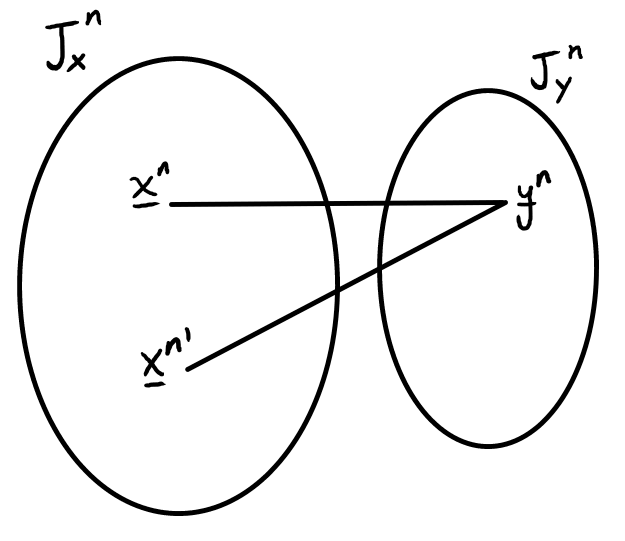
\includegraphics[width=0.35\textwidth]{lent/qi/2019/01/20190125_noisychannel1.png}
    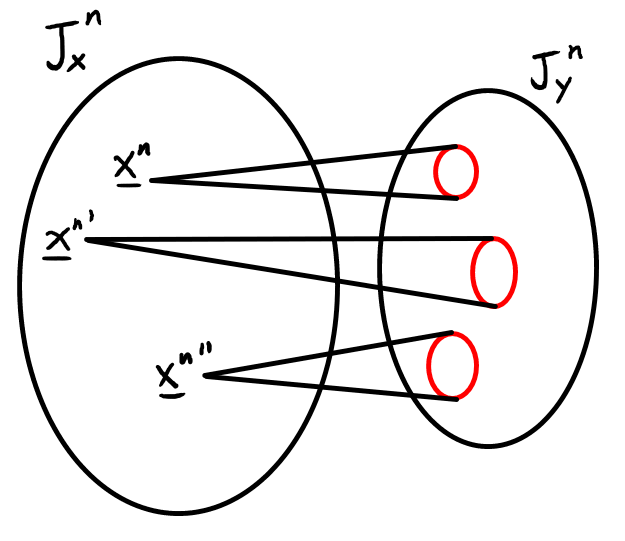
\includegraphics[width=0.35\textwidth]{lent/qi/2019/01/20190125_noisychannel2.png}
    \caption{In a noisy channel, it might be the case that multiple inputs map to the same output, as in the left set of ovals. Both $\underline{x}^n$ and $\underline{x}^n{}'$ have been mapped to the same $\underline{y}^n$ with some probability. However, Shannon tells us that certain codewords will be transmitted as disjoint regions (red ovals) after being sent through the channel, so those codewords can be reliably decoded after transmission.}
    \label{fig:noisychannel}
\end{figure}

We won't do the full proof of the theorem today, but we can introduce the setup. Suppose Alice has a message $[M]=\set{1,2,\ldots, M}$ she would like to send to Bob. She has a noisy channel $\mathcal{N}:J_X \to J_Y$ with some transition probabilities $p(\underline y^{n}| \underline x^{n})$.

%encoding-decoding Tikz figure
\begin{center}
    \begin{tikzpicture}[scale=2, node distance = 2.5cm]
        %make nodes
        \node [] (start) {};
        \node [block, right of=start] (encoding) {$\mathcal{E}_n$};
        \node [block, right of=encoding] (channel) {$\mathcal{N}$};
        \node [block, right of=channel] (decoding) {$\mathcal{D}_n$};
        \node [right of=decoding] (end) {};
        
        %make lines
        \path [line] (start) -- node[below] {$m\in M$} (encoding);
        \path [line] (encoding) -- node[below] {$x_m$} (channel);
        \path [line] (channel) -- node[below] {$y_m$} (decoding);
        \path [line] (decoding) -- node[below] {$m'$} (end);
    \end{tikzpicture}
\end{center}

\begin{enumerate}
    \item First, Alice can choose an encoding scheme $\mathcal{E}_n:[M]\to J_X^n$ where $\forall m\in [M], \mathcal{E}_n(m)=\underline x^{(n)} \in J_X^n$.
    \item She then sends her message through the channel $\mathcal{N}^{(n)}:x^{(n)}\to y^{(n)}$, producing some transmitted messages $y^{(n)}$ with some given probabilities.
    \item Bob receives the message and performs the decoding with $\mathcal{D}_n$ to get some decoded message $\mathcal{D}_n(\mathcal{N}^{(n)}(\mathcal{E}_n(M)))=m'$.
\end{enumerate}

Thus the \term{maximum probability of error} is
\begin{equation}
    \max{m\in [M]} P(\mathcal{D}_n(\mathcal{N}^{(n)}(\mathcal{E}_n(M))) \neq m) = p(\mathcal{E}_n,\mathcal{D}_n).
\end{equation}
We say that the \term{rate} is the number of the bits of the message transmitted per use of the channel. That is,
\begin{equation}
    R= \frac{\log M}{n}
\end{equation}
since $M \approx 2^{\lfloor nR \rfloor}.$

\begin{defn}
    We say that a rate is $R$ is \term{achievable} if there exists a sequence $(\mathcal{E}_n, \mathcal{D}_n)$ with $M=2^{nR}$ such that
    \begin{equation}
        \lim_{n\to \infty} p(\mathcal{E}_n,\mathcal{D}_n)= 0,
    \end{equation}
    i.e. the maximum probability of error tends to zero as $n$ goes to $\infty$.
\end{defn}

We make one final definition for today.
\begin{defn}
    The \term{channel capacity} is defined to be
    \begin{equation}
        C(\mathcal{N})=\sup \set{R: R\text{ is an achievable rate}},
    \end{equation}
    the maximum achievable rate for a channel.
\end{defn}

\subsection*{Non-lectured: m.b.s.c encoding}

For Example \ref{exm:mbsc}, we were asked to consider a binary channel $N$ with error probability $p$. That is, if we give it an input $x\in \set{0,1}$, we get an output $N(x)=y\in \set{0,1}$ such that $p(N(x)\neq x)=p$.

We came up with the following encoding scheme: send $0\mapsto 000$ and $1\mapsto 111$. To decode, we simply take a majority vote, e.g. $010$ was ``probably'' $000$, so the original message was $0$. Now how much better can we do with this redundancy? Let's consider the possible inputs, how they would be encoded, and how often they would be correct.

Suppose we want to send $0\mapsto 000$.
\begin{itemize}
    \item With probability $(1-p)^3$, none of the three bits are flipped and we get $000$ as the output. The process succeeds.
    \item With probability $3\times p(1-p)^2$, exactly one of the three bits is flipped. (The factor of $3$ comes from the fact that we could have flipped any of the three.) We still succeed.
    \item If two or three bits are flipped, we definitely fail.
\end{itemize}
By the symmetry of the problem, the success and failure probabilities are the same for $1\mapsto 111$.

Let's add this up to get the total success probability:
\begin{equation}
    (1-p)^3+3p(1-p)^2=(1+2p)(1-p)^2.
\end{equation}
When $p=1/2$, the success probability of our scheme is
\begin{equation}
    (1+2p)(1-p)^2=(2)(1/2)^2=1/2.
\end{equation}
We can nicely visualize this with the following graphic:
\begin{center}
    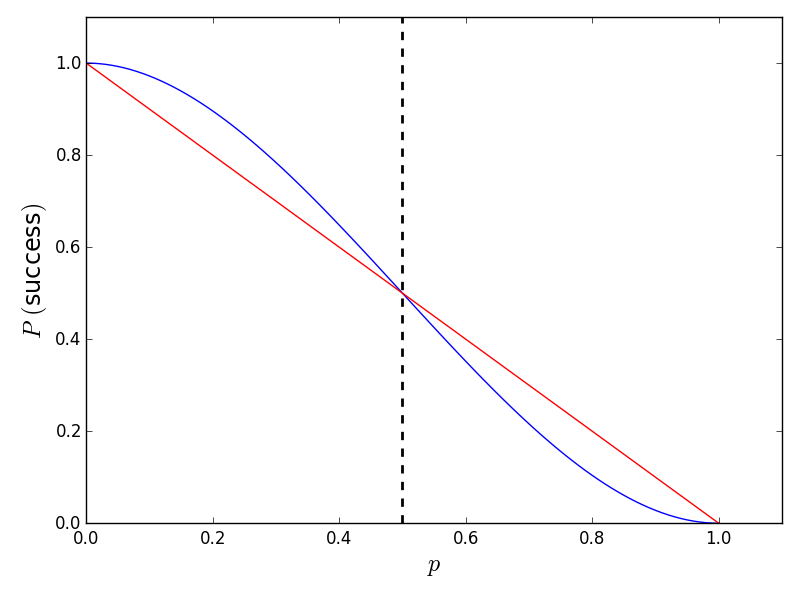
\includegraphics[width=0.5\textwidth]{2019/01/20190125_redundancy.png}
\end{center}
Here, the curved blue line is our three-bit scheme and the red line is the single-bit success probability $1-p$. For completeness, we can explicitly show that the crossover points occur when $P(\text{three bits})-P(\text{one bit})=(1+2p)(1-p)^2-(1-p)=0.$ Rewriting, we have $(1-p)(1-2p)p=0$, which clearly has zeroes at $p=0,1/2,1$. If we now take a derivative, we see that $\frac{d}{dp}\paren{P(\text{three bits})-P(\text{one bit})}|_{p=1/2}=1-6(1/2)+6(1/2)^2=-1/2,$ so $P(\text{three bits})>P(\text{one bit})$ for $p<1/2$.

\section{Monday, January 28, 2019}
    Last time, we began discussing the quantization of the string. We said that our approach would be to quantize the unconstrained first and then apply the quantum-ized constraint $T_{ab}=0$ on all physical states in the Hilbert space. We do this by imposing the conditions
\begin{equation}
    L_n \ket{\phi}=0, \quad n>0
\end{equation}
for $\ket{\phi}$ to be physical. Note that $\bar L_n\ket{\phi}=0$ as well-- for most of our theory, we'll get an exact copy of the behavior of the right-handed modes $L_n$ in the left-handed modes $\bar L_n$.

We also observed that our definition of $L_0$ was ambiguous in the quantum theory. In the other operators, we always had products of modes $\alpha_n$ with different harmonics $n$, but for $L_0$ there is an ordering ambiguity. We therefor impose the physical condition that
\begin{equation}
    (L_0-a)\ket{\phi}=0, \quad (\bar L_0 -a)\ket{\phi}=0
\end{equation}
where $a\in \RR$ quantifies this ordering ambiguity. We will see later (cf. BRST invariance) that the theory is consistent only if $D=26,a=1$. From now on we shall assume $a=1$.

It will be useful to define
\begin{equation}
    L_0^\pm = L_0 \pm \bar L_0,
\end{equation}
so that we have
\begin{equation}
    (L_0^+ -2)\ket{\psi}=0,\quad L_0^- \ket{\psi} = 0, \quad L_n \ket{\psi}=\bar L_n \ket{\psi}=0, n>0.
\end{equation}
These three conditions characterize physical states. Recall that $L_0=\frac{\alpha'}{4} p^2 + N, \bar L_0=\frac{\alpha'}{4} p^2 + \bar N$.

\subsection*{The spectrum} We'll start by looking at the lowest-lying modes of the theory. We haven't yet discussed the creation or destruction of strings, so the following discussion will, if you like, be centered on free propagators.

We begin by remarking that in our version of the theory, there are problems in the infrared which have to do with \term{tachyons}. These problems can be addressed in superstring theory, which is beyond the scope of this course.

The simplest state we can write down is the momentum eigenstate,
\begin{equation}
    \ket{k}=e^{ik\cdot x}\ket{0},
\end{equation}
with $k_\mu$ some four-vector of our choice and $x$ the center of mass coordinate for the string (i.e. the $x$ such that $X^\mu(\sigma, \tau)=x^\mu+p^\mu \tau+{}$oscillations).
The action of the center of mass momentum $p_\mu$ is then
\begin{equation}
    p_\mu \ket{k}= k_\mu \ket{k}.
\end{equation}

We could define a general state by a weighted sum of these momentum eigenstates,
\begin{equation}
    \ket{T}=\int d^Dk\, T(k) \ket{k},
\end{equation}
where $T(k)$ is a function of our choosing and we are working in $D$ dimensions. Now the $L_0^-\ket{\phi}=0$ condition imposes $N=\bar N$. This is called the ``level-matching'' condition. It turns out to be the only condition that relates the left-going and right-going modes-- otherwise, they are totally uncoupled.

If we look at $L_0^+$, we get the condition
\begin{equation}
    (L_0^+ -2)T(k)\ket{k}= \paren{ \frac{\alpha'}{2}p^2 + N +\bar N -2} T(k) \ket{k}=0,
\end{equation}
which tells us that $N=\bar N = 0$. Therefore
\begin{equation}
    (L_0^+ -2)T(k)\ket{k}= \paren{ \frac{\alpha'}{2}p^2-2} T(k) \ket{k}=0,
\end{equation}
which we can rewrite as a mass-shell condtion on the momentum space field $T(k)$:
\begin{equation}
    (k^2+M^2) T(k)=0\quad\text{where } M^2=-\frac{4}{\alpha'}.
\end{equation}
We notice that the field $T(k)$ is tachyonic, i.e. its mass squared is negative. (We use the mostly $+$ sign convention for the Minkowski metric.) Note that
\begin{equation}
    L_n\ket{T}=0 =\bar L_n\ket{T} \text{ for }n>0
\end{equation}
is satisfied trivially. A priori, tachyons need not sink our theory. It could be that we're just working relative to the wrong vacuum. This is an open question, though there are other reasons the bosonic string might not be quite the right model for our universe's physics. Having declared that superstring theory does provide some solution to this problem, we will pay it no more thought and move on.

\subsection*{Massless states}
Next, we consider states of the form
\begin{equation}
    \ket{\epsilon}=\epsilon_{\mu\nu}(k) \alpha_{-1}^\mu \bar \alpha_{-1}^\nu \ket{k},
\end{equation}
where we have included both $\alpha$ and $\bar \alpha$ to satisfy level-matching, and we have thrown in an $\epsilon$ in order to kill the free indices.

The condition $(L_0^+-2) \ket{\epsilon}=0$ gives $M^2=0$ since $N=\bar N = 1$. Note that $L_n \ket{\epsilon}=0$ is satisfied trivially for $n>1$ (and so is $\bar L_n \ket{\epsilon}=0$).

What about $L_1\ket{\epsilon}=0$? We have
\begin{align*}
    L_a \ket{\epsilon} &= \frac{1}{2} \sum_n \alpha_{1-n} \cdot \alpha_n \epsilon_{\mu\nu} \alpha_{-1}^\mu \bar \alpha_{-1}^\nu \ket{k}\\
    &= \epsilon_{\mu\nu}(k) \alpha_0 \cdot \alpha_1 \alpha_{-1}^\mu \bar \alpha_{-1}^\nu \ket{k}\\
    &=\sqrt{\frac{2}{\alpha'}} \epsilon_{\mu\nu} (k) k_\lambda \a_1^\lambda \a_{-1}^\mu \bar \a_{-1}^\nu \ket{k}\\
    &=\sqrt{\frac{2}{\a'}} \epsilon_{\mu\nu} (k) k_\lambda \paren{[\a_1^\lambda, \a_{-1}^\lambda]+\a_{-1}^\mu \a_1^\lambda} \bar \a_{-1}^\nu\ket{k}.
\end{align*}
We conclude that
\begin{equation}
    \epsilon_{\mu\nu}(k)k^\mu =0,
\end{equation}
so two states related by
\begin{equation}
    \epsilon_{\mu\nu}(k)\to \epsilon_{\mu\nu}(k) + k_\mu \xi_\nu
\end{equation}
are physically equivalent since $k^2=0$, with $\xi$ arbitrary. Similarly,
\begin{equation}
    \bar L_1\ket{\epsilon}=0 \implies k^\nu \epsilon_{\mu\nu}(k)=0.
\end{equation}
It is useful to decompose $\epsilon_{\mu\nu}(k)$ as follows:
\begin{equation}
    \epsilon_{\mu\nu}(k)=\tilde g_{\mu\nu}(k) + \tilde B_{\mu\nu}(k)+\eta_{\mu\nu} \tilde \phi(k),
\end{equation}
where $\tilde g_{\mu\nu}$ is traceless symmetric and $\tilde B_{\mu\nu}$ is antisymmetric. Now $\tilde g_{\mu\nu}(k)$ has the interpretation of a momentum space metric perturbation,
\begin{equation}
    \tilde g_{\mu\nu}(k) \sim \tilde g_{\mu\nu}(k) + k_\mu \xi_\nu + \xi_\mu k_\nu,
\end{equation}
which is simply (linearized) diffeomorphism invariance. What about this antisymmetric guy? We get a ``$B$-field'' which corresponds to a momentum spacetime field $\tilde B_{\mu\nu}=-\tilde B_{\nu\mu}$, where
\begin{equation}
    \tilde B_{\mu\nu} (k) \sim \tilde B_{\mu\nu}(k)+k_\mu \lambda_\nu - k_\nu \lambda_\mu.
\end{equation}
In spacetime this is a gauge invariance, where $B_{\mu\nu}\sim B_{\mu\nu} + \p_\mu \lambda_\nu - \p_\nu \lambda_\mu.$ Some older textbooks call this the notoph (which is nearly ``photon'' backwards).
    
\section{Wednesday, January 30, 2019}
    Today, we shall begin our discussion of quantum information theory. First, a quick review of Dirac's bra-ket notation-- we denote a vector in Hilbert space $\cH =\CC^d$ by
\begin{equation}
    \ket{v} = \begin{pmatrix}
    v_1\\ \vdots \\ v_d
    \end{pmatrix},
\end{equation}
and call this a \term{ket}. We also have the dual vectors (row vectors, if you like), called \term{bras}. such that
\begin{equation}
    \bra{v}=(v_1^*, \ldots, v_d^*).
\end{equation}
The braket notation provides us with a natural inner product:
\begin{equation}
    (u,v)=\braket{u}{v}=\sum_{i=1}^d u_i^* v_i.
\end{equation}
This space also comes equipped with an outer product, $\ket{u}\bra{v}$, which is the matrix
\begin{equation}
    \ket{u}\bra{v} =\begin{pmatrix}
    u_1 v_1^* &\ldots&\\
    \vdots\\
    u_d v_1^* &\ldots &u_d v_d^*
    \end{pmatrix}.
\end{equation}
We can then take an orthonormal basis (onb) for $\cH$, which we denote by $\set{\ket{e_i}}$ with $\braket{e_i}{e_j}=\delta_{ij}$. Note that for any basis of $\cH$, we can write the identity matrix as
\begin{equation}
    I=\sum_{i=1}^d \ket{e_i}\bra{e_i}.
\end{equation}
There is a nice basis $\ket{e_1}=\begin{pmatrix}1\\0\\\vdots\\0\end{pmatrix}$ we can write down,
so that for a general basis $\set{\ket{f_i}}_{i=1}^d$ related to the original by a unitary $U$, we find that
\begin{equation}
    \sum_{i=1}^d \ket{f_i}\bra{f_i}=\sum_{i=1}^d U \ket{e_i} \bra{e_i} U^\dagger = U I U^\dagger =UU^\dagger = I.
\end{equation}

Now in classical information, our simplest system was a binary bit, a system taking values $0$ and $1$. For quantum information theory, we have a \term{qubit}, a two-level system represented by a Hilbert space with $\cH=\CC^2$ and basis vectors $\set{\ket{0},\ket{1}}$ or equivalently $\set{\ket{\uparrow},\ket{\downarrow}}.$ Physically, these could be the spin states of an electron or perhaps the polarizations of a photon.

Now, it is obvious that any state in Hilbert space can be decomposed in the basis of our choice, i.e.
\begin{equation}
    \ket{\psi}=a\ket{0}+b\ket{1},
\end{equation}
with $a,b\in \CC$. We shall require that our states are normalized under this inner product, so that
\begin{equation}
    1=\braket{\psi}{\psi}=|a|^2+|b|^2,
\end{equation}
which means that $|a|^2$ and $|b|^2$ have the interpretation of probabilities.

We also have some important operators on Hilbert space. These are the Pauli matrices%fill in the pauli matrices
$\sigma_0,\sigma_x,\sigma_y,\sigma_z$. As it turns out, these operators form a basis. Note that we have a set of self-adjoint $2\times 2$ complex matrices
\begin{equation}
    B_{SA}(\CC^2)=\set{A\in B(\cH): A=A^\dagger},
\end{equation}
and we can write a general matrix $M\in M_2 /M_{sa}$ in terms of the Pauli matrices,
\begin{equation}
    M=\frac{1}{2}(x_0 \sigma_0 +\vec x \cdot \gv \sigma),
\end{equation}
where $\vec x=(x_1,x_2,x_3)\in \RR^3$.

\subsection*{Spectral decomposition}
The spectral decomposition says that we can write a matrix in terms of its eigenvalues,
\begin{equation}
    A=\sum_{i=1}^d \lambda_i \ket{e_I}\bra{e_i},
\end{equation}
such that $A\ket{e_i}=\lambda_i \ket{e_i}$. Sometimes, we say that the eigenvalue decomposition is written in terms of projectors instead,
\begin{equation}
    A=\sum_{i=1}^m \lambda_i \Pi_i
\end{equation}
where $\Pi_i$ projects onto some basis.

Given a self-adjoint operator $A=A^\dagger$ and a nice function $f$, what is the value $f(A)$? Note that $A$, being self-adjoint, can be diagonalized by a unitary. Thus
\begin{equation}
    A_d = UAU^\dagger \implies A = U^\dagger A_d U,
\end{equation}
so that
\begin{equation}
    f(A)=U^\dagger \begin{pmatrix}
    f(\lambda_1) && \\
    & \ddots & \\
    && f(\lambda_d)
    \end{pmatrix}.
\end{equation}
Thus for example
\begin{equation*}
    f(A)=e^{iA}=I + iA +\frac{i^2}{2!}+\ldots.
\end{equation*}

\subsection*{QM postulates}
We consider the following postulates of quantum mechanics, which will in fact be qualified by the fact we are working in an open system.
\begin{enumerate}
    \item The state of a (closed) system is given by a ray in $\cH$, i.e. a vector defined up to a global phase. Thus we cannot distinguish a state $\ket{\psi}$ and $e^{i\phi}\ket{\psi}$ by any physical measurement. We traditionally take a representative of this equivalence class, $\ket{\psi}.$
\end{enumerate}
For an open system $A$, consider a system which is in states $\ket{\psi_i}$ with some coefficients $p_i, i=1,\ldots, m$. The state is characterized by an ensemble
\begin{equation}
    \set{p_i,\ket{\psi_i}}_{i=1}^m.
\end{equation}
Note that these $\ket{\psi_i}$s need not be mutually orthogonal,
\begin{equation}
    \braket{\psi_i}{\psi_j}\neq \delta_{ij},
\end{equation}
and moreover this is \emph{not} a superposition but a statistical mixture. A superposition is a pure state where the state is normalized and can be written as 
\begin{equation}
    \ket{\Psi}=\sum_{i=1}^d a_i \ket{\phi_i}.
\end{equation}

So a statistical mixture is instead described by a \term{density matrix} (or density operator). We could write our ensemble as
\begin{equation}
    \rho \equiv \sum_{i=1}^m p_i \ket{\psi_i} \bra{\psi_i},
\end{equation}
noting that the $\ket{\psi_i}$s in general \emph{need not be orthogonal}.
\begin{defn}
    A \term{density matrix} on $\cH$ ($\dim \cH = d$) is an operator $\rho$ with the following properties:
    \begin{itemize}
        \item $\rho \geq 0$, i.e. $\rho$ is positive semi-definite, $\bra{\phi}\rho \ket{\phi}\geq 0,$ which implies that $\rho=\rho^\dagger$.
        \item $\Tr \rho =1$ (which gives it a probabilistic interpretation).
    \end{itemize}
\end{defn}
Let us remark that $\rho$ is hermitian and therefore admits a spectral decomposition, i.e.
\begin{equation}
    \rho = \sum_{j=1}^d \lambda_j \ket{e_j}\bra{e_j}
\end{equation}
in terms of an orthonormal basis. Thus
\begin{equation}
    \rho=\sum_{i=1}^m p_i \ket{\psi_i}\bra{\psi_i} = \sum_{j=1}^d \lambda_j \ket{e_j} \bra{e_j}.
\end{equation}
We will prove on Examples Sheet 2 that the set
$\mathcal{D}(\cH)$ of density matrices is a complex set.

\subsection*{Pure and mixed states} 
Consider a density matrix
\begin{equation}
    \rho = \sum p_i \ket{\psi_i}\bra{\psi_i},
\end{equation}
and suppose for example that $p_2=1, p_i=0 \forall i\neq 2$. Then
\begin{equation}
    \rho=\ket{\psi_2}\bra{\psi_2}.
\end{equation}
This is very nice, because we know precisely the state of the system (or equivalently the outcome of applying the operator $\rho$). We call this a \term{pure state}, referring either to the vector $\ket{\psi_2}$ or the operator $\ket{\psi_2}\bra{\psi_2}$. Otherwise, $\rho$ is a \term{mixed state}.

A pure state will have $\rho^2 = \rho$, so we can define the \term{purity} of a state by $\Tr \rho^2$. Conversely, we can define a completely mixed state by
\begin{equation}
    \rho = I/d=\frac{1}{d} \sum_{i=1}^d \ket{e_i} \bra{e_i},
\end{equation}
such that a completely mixed state has purity $1/d$ (where we get a factor of $d$ from taking the trace of $I$).

In classical probability, we remark that the convex set of probability distributions forms a \term{simplex}.

Now let's briefly discuss the expectation value of an observable (self-adjoint operator) in $B(\cH)$. For a state $\rho$, we define the expectation value to be
\begin{equation}
    \phi(A) \equiv \avg{A}_\rho =\Tr(A \rho).
\end{equation}
This is a linear normalized functional--
\begin{itemize}
    \item $\phi(aA +b B) = a\phi(A) + b\phi(B)$
    \item $\phi(A)\geq 0$ with equality when $A=I$.
\end{itemize}
    
\section{Friday, February 1, 2019}
    Let us now continue our discussion of path integral quantization. Heuristically, we'll \begin{verbatim}import\end{verbatim} the details of path integral quantization and see what works out. We want to understand how to make sense of expressions like
\begin{equation}
    \int \cD h \cD X \,e^{iS[h,X]}
\end{equation}
where we are integrating over the space of metrics $h_{ab}$ and embedding fields $X^\mu$s. When we do this calculation, we have to be careful not to overcount-- there is a huge diffeomorphism symmetry and a Weyl symmetry in our theory relating physically equivalent states. If this path integral is to give us anything physically meaningful, we need to ``quotient out'' by the space of diffeomorphisms and Weyl transformations.

We would like to split the integral over all $h_{ab}$ into integrals over physically inequivalent $h_{ab}$ and those related by gauge transformations. Schematically,
\begin{equation}
    \cD h = \cD h_{\text{phys}}\times \mathcal{J}\cD h_{\text{Diff}\times \text{Weyl}},
\end{equation}
where $\mathcal{J}$ is a Jacobian factor whose importance we'll see in the following example.

\begin{exm}
    As a toy example, consider the following integral:
    \begin{equation*}
        \int dxdy\, e^{-(x^2 +y^2)}.
    \end{equation*}
    But notice that $x^2+y^2$ is invariant under rotations about the origin. When we pass to polar coordinates, the $\theta$ angular integral becomes totally trivial, so we might really be interested in this integral modulo rotations. Thus our integral can be rewritten
    \begin{equation*}
        \int d\theta \int dr \, re^{-r^2}.
    \end{equation*}
    This $\int d\theta$ will always give us a factor of $2\pi$ (the  ``volume'' of an orbit of the rotation group)-- the real interest is in the $dr$ integral.
\end{exm}

In this example, we needed the Jacobian of the coordinate transformation: $dxdy=rdr d\theta$. The same is true of our path integral. Formally, we will take
\begin{equation}
    \frac{1}{|\text{Diff}|\times |\text{Weyl}|}\int \cD h \cD X = \int \cD h_{\text{phys}}\cD S_{\text{phys}} \,\mathcal{J},
\end{equation}
where $\mathcal{J}$ is now a functional determinant and $|\text{Diff}|, |\text{Weyl}|$ represents the orbits of diffeomorphisms and Weyl transformations.
%
In the same way we could write
\begin{equation}
    \sqrt{\frac{\pi}{\det M}}=\int_V dx \,e^{-(x,Mx)},
\end{equation}
we will write $\mathcal{J}$ as a functional integral,
\begin{equation}
    \cJ =\int \cD b \cD c\, e^{-S[b,c]}.
\end{equation}

\subsection*{Global properties of the worldsheet} We need to know more about what type of worldsheets appear in the path integral. This will take us on a crash course through Riemann surfaces.

We have looked at 2-dimensional Riemannian manifolds $(\Sigma,h)$ modulo Weyl transformations. The set of Riemannian manifolds modulo Weyl transformations is known as \term{Riemann surfaces}. Quotienting out by diffeomorphisms is assumed. Note that worldsheets are Riemann surfaces.

We'll state a number of results without proof, though some of them are not too hard to prove-- for more detail, see Farkas and Kra, and also Donaldson.

The first idea we'll consider is the \term{worldsheet genus}. For Riemann surfaces without boundary (i.e. a closed string, neglecting the initial and final string states), the relevant topological data is encoded in the \term{Euler characteristic},
\begin{equation}
    \chi = \frac{1}{4\pi} \int_\Sigma d^2 \sigma \,\sqrt{h} R(h).
\end{equation}
Here, $R(h)$ is the Ricci scalar with respect to the worldsheet metric $h$. The Euler characteristic captures the idea that while we can locally make the metric look however we want, in general there will be obstructions to globally bringing the metric to a required form. The \term{genus} $g$ is given by
\begin{equation}
    \chi = 2-2g,
\end{equation}
and informally counts the ``number of holes in $\Sigma$.'' Why we care is because the genus is a topological invariant. We can't change the number of holes in a Riemann surface under smooth maps.

\subsection*{Moduli space of Riemann surfaces} For a given genus $g$, the space of metrics on $\Sigma_g$ modulo Weyl and diffeomorphisms is a finite-dimensional space called the \term{moduli space}. Schematically,
\begin{equation*}
    \cM_g = \frac{\set{\text{metrics }h_{ab}}}{\set{\text{Diff}}\times \set{\text{Weyl}}}.
\end{equation*}
Both the numerator and denominator here are infinite dimensional, but our saving grace will be the following fact-- the integral itself is finite-dimensional.

A useful result is the following: let $s$ be the real dimension of the moduli space $\cM_g$. Then
\begin{equation}
    s=\dim \cM_g =\begin{cases}
    0, & g=0\\
    2, & g=1\\
    6g-6, & g\geq 2.
    \end{cases}
\end{equation}

\begin{exm}
    Given a metric $\hat h_{ab}$ on a $g=0$ surface, we can bring any metric to the form $e^{2w}\hat h_{ab}$. This is not the case for a torus ($g=1$). We can build a torus by imposing identifications on $\CC,$ i.e. under the equivalence relation
    \begin{equation}
        z\sim z + n \lambda_1 + m\lambda_2,
    \end{equation}
    where $n,m\in \ZZ$ and $\lambda_1,\lambda_2$ specify the ``dimensions'' of the torus.
    
    One can show that the ratio $\tau\equiv \lambda_1/\lambda_2$ is Diff and Weyl invariant. However, we can always choose $\lambda_1,\lambda_2$ such that $\Im (\tau)\geq 0$. We also get a metric
    \begin{equation}
        ds^2=\abs{dz+\tau d\bar z}^2.
    \end{equation}
    If we transform $\begin{pmatrix}\lambda_1 \\lambda_2\end{pmatrix}\to U\begin{pmatrix}\lambda_1 \\lambda_2\end{pmatrix}$ for some matrix $U$, then we can undo that change by also changing the equivalence relation numbers $(n,m)\to (n,m)U^{-1}$. For $n,m$ to be integers under any such transformation, we require the entries of $U$ to all be integers, i.e. $U\in SL(2,\ZZ)$.
    
    Our moduli space is
    \begin{equation}
        \cM_1 = \frac{UHP}{SL(2,\ZZ)},
    \end{equation}
    with $UHP$ the upper half-plane, $\tau,\Im \tau \geq 0$.
\end{exm}

\section{Monday, February 4, 2019}
    We've started our lightning tour of the theory of Riemann surfaces. Soon, we'll see the emergence of our first scattering amplitudes.

\subsection*{Conformal Killing vectors} Recall from \emph{General Relativity} that Killing vectors are very special objects which represent symmetries of the metric. In the language of Lie derivatives, a vector $K$ is a Killing vector if the Lie derivative of the metric with respect to $K$ is trivial, $\cL_K g =0$.%
    \footnote{In terms of covariant derivatives, $\nabla_a K_b + \nabla_b K_a = 0$.
    }
\term{Conformal Killing vectors} (CKV) generalize this idea. A conformal Killing vector generates diffeomorphisms that preserve the metric up to Weyl transformations.

Our gauge transformations are
\begin{gather}
    \delta_V h_{ab} = \nabla_a V_b +\nabla_b V_a\\
    \delta_\omega h_{ab} = 2\omega h_{ab}.
\end{gather}
We are interested in $V^a$ such that
\begin{equation}
    \delta_{CK} h_{ab}=\nabla_a V_b + \nabla_b V_a + 2\omega h_{ab}=0.
\end{equation}
Note the covariant derivatives are taken with respect to the metric $h_{ab}$. Taking the trace, we have equivalently
\begin{equation}
    2(\nabla_a V^a) +4\omega = 0 \implies \omega = -\frac{1}{2} (\nabla_a V^a),
\end{equation}
so $V^a$ is a conformal Killing vector if
\begin{equation}
    \delta h_{ab} = \nabla_a V_b + \nabla_b V_a - h_{ab}(\nabla_c V^c)=0.
\end{equation}
We define
\begin{equation}
    (Pv)_{ab}\equiv \nabla_a V_b+ \nabla_b V_a -h_{ab}(\nabla_c V^c)
\end{equation}
so that $V^a$ is a conformal Killing vector if $V^a\in \text{Ker}P$.

Why have we introduced these? For closed Riemann surfaces of genus $g$, the (real) dimension of the conformal Killing group (CKG), i.e. the subgroup of diffeomorphisms generated by the conformal Killing vectors, is known: it is
\begin{equation}
    \kappa =|\text{CKG}|=\begin{cases}
        6, & g=0\\
        2, & g=1\\
        0, & g \geq 2.
    \end{cases}
\end{equation}
On the sphere (think of this as $\CC$ with the point at $\infty$), the CKVs generate the transformations
\begin{equation}
    z \to \frac{az+b}{cz+d}
\end{equation}
and similarly for $\bar z$, where $a,b,c,d\in \CC$ and $ad-bc=1$. This is in fact the \href{https://en.wikipedia.org/wiki/M\%C3\%B6bius_transformation}{M\"obius group} from complex analysis. We have four parameters and one algebraic constraint on complex values (hence two real constraints). Therefore we shall fix the conformal Killing symmetry by requiring that the $V^a$ vanish at three distinct points on $\Sigma$ (i.e. imposing six real constraints, since each point on $\Sigma$ comes with two coordinates).

We'll need one more mathematical preliminary before moving forward. This is the \term{modular group.} First, observe that the diffeomorphism group on the Riemann surface $\Sigma_g$ is in general not connected. Let us therefore define something useful-- call the connected set of diffeomorphisms that includes the identity $\text{Diff}_0$. The modular group $\cM_g$ is then
\begin{equation}
    \cM_g =\frac{\text{Diff}}{\text{Diff}_0}.
\end{equation}
For example, for the torus we have $\cM_1=\text{SL}(2:\ZZ)$.

Then the moduli space $M_g$ can be written schematically as
\begin{equation}
    M_g = \frac{\set{\text{metrics}}}{\set{\text{Diff}}\times \set{\text{Weyl}}}=\frac{\set{\text{metrics}}}{\set{\text{Diff}_0}\times \set{\text{Weyl}}}/\cM_g.
\end{equation}
We often call the space
\begin{equation}
    \mathcal{T}_g= \frac{\set{\text{metrics}}}{\set{\text{Diff}_0}\times \set{\text{Weyl}}}
\end{equation}
the Teichm\"uller space. In this notation, $M_g= \mathcal{T}_g/\cM_g$.

\subsection*{The Faddeev-Popov determinant} When we do path integrals, it's usually desirable to check our answer by other means, since path integrals have a way of hiding divergences which we as self-respecting physicists ought to care about. Happily, this will be possible for the following quantity we are about to define.

The idea is to choose a ``gauge slice'' through the space of metrics on $\Sigma_g$. That is, we choose a gauge such that the metric on the worldsheet $h_{ab}$ takes some nice form, $h_{ab}=\hat h_{ab}$ (often diagonal), such that $\text{Diff}_0\times\text{Weyl}$ orbits then take us everywhere else in our space of metrics. We formally define the \term{Fadeev-Popov determinant} as
\begin{equation}
    1=\Delta_{FG}(\hat h)\int_{\text{Diff}_0 \times \text{Weyl}} \cD(\delta h) \delta[h-\hat h] \prod_i \delta(v(\hat \sigma_i)),
\end{equation}
where $\delta[h-\hat h]$ can be thought of as a ``delta functional'' and $\sigma_i$ indicates points on our worldsheet $\Sigma_g$ where the CKVs vanish (in order to fix the CKG). We can think of this determinant in analogy to how $\delta(f(x))\sim \frac{\delta x}{|f'(x_i)|}$ where $f(x_i)=0.$

In more detail, we may write
\begin{equation}
    1=\Delta_{FG}(\hat h) \int_{\mathcal{T}} d^s t \int \cD \omega \cD v \delta[h_{ab}-\hat h_{ab}] \prod_i \delta(v(\hat \sigma_i)),
\end{equation}
where the $d^s t$ integral is taken in Teichm\"uller space and our path integral is now written explicitly over the space of variations of $h$.

We will now write the delta functions and delta functions as integrals and functional integrals. Let us introduce numbers $\zeta^i_a$ and fields $\beta^{ab}(\sigma,\tau)$ such that
\begin{equation}
    1=\Delta_{FG}(\hat h) \int_{\mathcal{T}} d^s t \int \cD \omega \cD v \paren{d^\kappa \zeta^i_a \cD \beta \exp(i(\beta|h-\hat h)+i\zeta^i_a v^a (\hat \sigma_i)},
\end{equation}
where the inner product $(\beta|h-\hat h)$ is defined to be
\begin{equation}
    (\beta|h-\hat h) = \int_\Sigma d^2 \sigma \sqrt{|h|}\beta^{ab}(h_{ab}-\hat h_{ab})
\end{equation}

We can write $h_{ab}-\hat h_{ab}=\delta_{ab}$ as
\begin{align*}
    \delta h_{ab}&=\underbrace{\nabla_a v_b + \nabla_b v_a}_{\text{Diffeos}} +\underbrace{2\omega h_{ab}}_{\text{Weyl}}+\underbrace{t^I \p_I h_{ab}}_{\text{moduli}}\\
        &= (Pv)_{ab} +2(\omega+\nabla_c v^c)h_{ab} +t^I \p_I h_{ab}\\
        &= (Pv)_{ab}+2\bar \omega h_{ab} +t^I \mu_{Iab}
\end{align*}
where $(Pv)_{ab}$ is as defined before, $\mu_{Iab}=\p_Ih_{ab}-\text{trace}$, and $\bar \omega$ contains the residual trace terms.
    
\section{Wednesday, February 6, 2019}
    Last time, we introduced maximally entangled states. As it turns out, these states have a few interesting properties. Recall that such states are defined on composite Hilbert spaces such that for
\begin{equation}
    \cH_A \otimes \cH_B \simeq \CC^d \otimes \CC^d
\end{equation}
equipped with a (fixed) onb for $\CC^d$ given by $\set{\ket{i}}_{i=1}^d$, a maximally entangled state is then a state which is written
\begin{equation}
    \ket{\Omega}=\frac{1}{\sqrt{d}} \sum_{i=1}^d \ket{i}\ket{i}.
\end{equation}
\begin{itemize}
    \item Every MES $\ket{\Phi}\in \CC^d \otimes \CC^d$ can be written in the form
    \begin{equation}
        \ket{\Phi}=(I_d \otimes U) \ket{\Omega}
    \end{equation}
    for some unitary $U$. One should check explicitly%
        \footnote{The proof is quick.
        \begin{align*}
            \Tr_2(\kb{\Phi}{\Phi})&= \Tr_2 \paren{(I\otimes U) \frac{1}{\sqrt{d}}\sum_i \ket{i}\ket{i}}\paren{\frac{1}{\sqrt{d}} \sum_j \bra{j} \bra{j} (I\otimes U^\dagger)}\\
                &= \frac{1}{d}\sum_{i,j} \kb{i}{j} \Tr(U\kb{i}{j} U^\dagger)\\
                &= \frac{1}{d}\sum_{i,j} \kb{i}{j} \Tr(\kb{i}{j} U^\dagger U)\\
                &=\frac{1}{d} \sum_{i,j} \kb{i}{j} \delta_{ij}\\
                &= \frac{I}{d}.
        \end{align*}
        The proof for tracing over the first subsystem is almost the same. Strictly, what this shows is that every state of this form is maximally entangled. We haven't shown that every maximally entangled state admits this form.
        }
    that
    \begin{equation}
        \Tr_2 \ket{\Phi}\bra{\Phi}=\frac{I}{d}\text{ and }\Tr_1 \ket{\Phi}\bra{\Phi}=\frac{I}{d}.
    \end{equation}
    \item Lemma: for any $A,B\in B(\CC^d),$
    \begin{itemize}
        \item $\bra{\Omega}A\otimes B\ket{\Omega}=\frac{1}{d}\Tr(A^T B)$, where transposition is done in the basis $\set{\ket{i}}_{i=1}^d$.
        \item $(A\otimes I)\ket{\Omega}=(I\otimes A^T)\ket{\Omega}$, a property we shall call ``ricochet.'' The proofs of these lemmas are an exercise, and are done at the end of this lecture's notes.
        %We can do this by writing
        %\begin{gather*}
        %    A=\sum_{i,j} a_{ij}\ket{i}\bra{j}\\
        %    B=\sum_{k,l} a_{kl}\ket{k}\bra{l}\\
        %    A^T=\sum_{i,j} a_{ji}\ket{i}\bra{j}.
        %\end{gather*}
        %and computing explicitly.
    \end{itemize}
    \item We can write down a purification $\rho$ of $\ket{\Omega}$: we claim it is
    \begin{equation}
        \ket{\Psi}=\sqrt{d}(\sqrt{\rho}\otimes I) \ket{\Omega}.
    \end{equation}
    Let us check:
    \begin{align*}
        \ket{\psi}\bra{\psi}&=d\sqrt{\rho} \otimes I \ket{\Omega}\bra{\Omega} \sqrt{\rho}\otimes I\\
            &= \sum_{i,j}\sqrt{\rho}\ket{i}\bra{j}\sqrt{\rho} \ket{i}\bra{j}.
    \end{align*}
    Tracing over the second system, $\ket{i}\bra{j}=\delta_{ij}$, so the partial trace is then
    \begin{equation}
        \Tr_2 \ket{\psi}\bra{\psi} = \sqrt{\rho} \sum_i \ket{i}\bra{i} \sqrt{\rho} = \rho.
    \end{equation}
    \item Every bipartite pure state $\ket{\psi}\in \cH_A \otimes \cH_B$ can be written in the form
    \begin{equation}\label{bipartitedecomp}
        \ket{\psi}=(I\otimes R) \ket{\Omega}
    \end{equation}
    for some operator $R$.
    \begin{proof}
        Let $\ket{\psi}=\ket{\psi_{AB}}=\sum \lambda_i \ket{i_A}\ket{i_B},$ by the Schmidt decomposition. Let $V,W$ be isometries such that
        \begin{gather}
            V\ket{i}=\ket{i_A}\forall i ; \quad V:\CC^d \to \cH_A\\
            W\ket{i}=\ket{i_B}\forall i; \quad W:\CC^d \to \cH_B.
        \end{gather}
        The proof is constructive. Choose $R \equiv W Q V^T$, where $Q$ is defined in terms of the Schmidt coefficients,
        \begin{equation}
            Q=\sum \sqrt{d} \lambda_j \ket{j}\bra{j}.
        \end{equation}
        Let us look at the RHS of \ref{bipartitedecomp}. For this choice of $R$, it is
        \begin{align*}
            &=(I\otimes WQV^T) \ket{\Omega}\\
            &=(I\otimes W)(I\otimes Q)(I\otimes V^T)\ket{\Omega}\\
            &=(I\otimes W)(I\otimes Q)(V\otimes I)\ket{\Omega}\\
            &= (V\otimes W)(I\otimes Q) \ket{\Omega}\\
            &= (V\otimes W) \frac{1}{\sqrt{d}} \sum_i \ket{ i}\otimes Q\ket{i} \sum_j \sqrt{d} \lambda_j \ket{j}\bra{j}\bra{i}\\
            &=(V\otimes W) \sum_i \lambda_i \ket{i}\otimes \ket{i}\\
            &= \sum \lambda_i \ket{i_A} \ket{i_B}.\qedhere
        \end{align*}
        Here, we have used the ``ricochet'' property to interchange $I\otimes V^T$ to $V\otimes I$, and moved $V\otimes I$ through $I\otimes Q$ since they act on independent parts of the composite system.
    \end{proof}
\end{itemize}

\subsection*{Time evolution of open systems}
Question: what is the most general description of the dynamics of an \emph{open} quantum system? Answer: it is given by a linear \term{completely positive trace-preserving} (CPTP) map. The advantage of such a map is that it gives us a description of the effect of \emph{any} allowed physical process on your system, including operations like measurement. In particular, it also allows us to describe discrete state changes.

As all reasonable evolution operators should be linear, we will usually omit this from the description and just speak of a CPTP map. We can also reasonably call this a \term{quantum operator} or a \term{quantum channel}. That is, we have a map $\Lambda:\cD(\cH)\to \cD(\cH)$, e.g. it takes the density matrix $\rho$ from $\rho\mapsto \Lambda(\rho)=\rho'$. We call this a \term{superoperator} because it is a map from operators to operators.

\begin{exm}
    We've constructed a general description of open quantum systems, but it should include our previous description of closed quantum systems as a special case. Take $\Lambda$ to be a unitary transformation, such that
    \begin{equation}
        \rho'=\Lambda(\rho)=U\rho U^\dagger.
    \end{equation}
    
    
\end{exm}
Let us now unpack some of the properties of CPTP maps.
\begin{itemize}
    \item This map satisfies linearity:
    \begin{equation*}
        \Lambda(a\rho_1 +b\rho_2) = a\Lambda(\rho_1) + b\Lambda(\rho_2).
    \end{equation*}
    We want our CPTP maps to be linear so that we can interpret mixed state density matrices in a probabilistic way. That is, if we have some distribution of density matrices $\rho_i$ given with some probabilities $p_i$ (i.e. a set $\set{p_i,\rho_i}_{i=1}^m$, then we can describe the system as a new density matrix
    \begin{equation*}
        \sigma=\sum_{i=1}^m p_i \rho_i,
    \end{equation*}
    and thus the map $\Lambda$ should also represent a valid map on the full system $\sigma$:
    \begin{equation*}
        \Lambda(\sigma)=\sum_{i=1}^m p_i \Lambda(\rho_i).
    \end{equation*}
    \item Positivity: for $\rho\geq 0, \rho' = \Lambda(\rho) \geq 0$. We say $\Lambda$ is a positive (or positivity-preserving) map if
    \begin{equation}
        \Lambda(A)\geq 0 \forall A \geq 0.
    \end{equation}
    \item $\Lambda$ must be trace-preserving, i.e. for $\rho$ with $\Tr \rho =1$, we want 
    \begin{equation}
        \Tr (\Lambda \rho)=\Tr \rho'=1.
    \end{equation}
\end{itemize}
These conditions are necessary, but not sufficient. In fact we, require $\Lambda$ to be \term{completely positive}, as we'll define now. 
\begin{defn}
    Let $\Lambda:\cD(\cH_A)\to \cD(\cH_A')$, where $\cH_A$ is the Hilbert space of this system. Consider an extension of $\cH_A$ to the bigger space $\cH_A \otimes \cH_B$. That is, we add another system $B,$ called the ancilla or (for obvious reasons) the environment. 

    Note that $I_B$ is the identity operator on $B$, i.e. $I_B\in \cB(\cH_B)$, whereas $id_B$ is the superoperator $\cB(\cH_B)\to \cB(\cH_B)$ such that $id_B Q=Q \,\forall Q\in B(\cH_B).$ We then say that $\Lambda$ is \term{completely positive} if $\Lambda \otimes id_B$ is positive for all such extensions.
\end{defn}
For instance, suppose the composite system $AB$ is initially in a state $\rho_A\otimes \omega_B$. Thus a completely positive map yields a state
\begin{equation}
    (\Lambda \otimes id_B)(\rho_A \otimes \omega_B)=\sigma_{AB},
\end{equation}
where $\sigma_{AB}$ is guaranteed to be a legitimate state of the composite system $AB$.

\begin{exm}
    Let $\Lambda$ be the transposition map. This is certainly positive:
    \begin{equation}
        \Lambda \equiv T: \rho \to \rho^T.
    \end{equation}
    That is, if $\rho$ had no negative eigenvalues, then transposition will preserve the eigenvalues and therefore preserve positivity.
    
    We will now show that there exists a composite state which is positive, but not positive after the application of $\Lambda \otimes id_B$. Let the composite system $\cH_A\otimes \cH_B$ with $\cH_A,\cH_B\simeq \CC^d$ be described by the density matrix
    \begin{equation}
        \rho_{AB}=\ket{\Omega}\bra{\Omega}
    \end{equation}
    where
    \begin{equation}
        \ket{\Omega}=\frac{1}{\sqrt{d}} \sum_{i=1}^d \ket{i}\ket{i}
    \end{equation}
    is a MES. Now we hit the first part with the transpose:
    \begin{align*}
        (\Lambda \otimes id_B)\ket{\Omega}\bra{\Omega} &= \frac{1}{d} \sum T(\ket{i}\bra{j}\otimes \ket{i}\bra{j}\\
        &= \frac{1}{d} \sum \ket{j}\bra{i} \otimes \ket{i}\bra{j} \equiv \tilde \rho.
    \end{align*}
    Now we ask whether $\tilde \rho \geq 0.$ The factor $d$ certainly doesn't change the positivity of the state, so take $Q\equiv d\tilde \rho$ and consider its action on some states $\ket{\phi}=\sum_k a_k \ket{k},\ket{\psi}=\sum_l b_l \ket{l}.$ Then
    \begin{align*}
        Q(\ket{\phi}\otimes \ket{\psi}) &= \paren{\sum \ket{j}\bra{i} \otimes \ket{i}\bra{j}}\paren{\sum a_k \ket{k} \otimes \sum b_l \ket{l}}\\
        &= \sum_{i,j} a_i \ket{j} \otimes b_j \ket{i}\\
        &=\sum_j b_j \ket{j} \otimes \sum_i a_i \ket{i} = \ket{\psi}\otimes \ket{\phi}.
    \end{align*}
    What we see is that $Q$ has swapped the states between the Hilbert spaces,
    \begin{equation}
        Q(\ket{\phi}\otimes \ket{\psi}) =\ket{\psi}\otimes \ket{\phi} \implies Q^2=I.
    \end{equation}
    This tells us that the eigenvalues of $Q$ are $\pm 1$, which means that we have constructed an operator which is positive but not completely positive.
\end{exm}

\subsection*{Non-lectured aside: extra proofs}
These proofs were originally footnotes, but I thought it might be useful to collect them here at the end of the lecture to avoid clutter.

\begin{proof}
    Trace and $\ket{\Omega}$: we show that $\bra{\Omega}A\otimes B\ket{\Omega}=\frac{1}{d}\Tr(A^T B)$.
    
    Note that by the usual laws of matrix multiplication, if $A=a_{ij}\ket{i}\bra{j}$ and similarly $B=b_{ij}\ket{i}\bra{j}$, then $A^TB=a_{ji}B_{jl}\ket{i}\bra{l}$ and so 
    \begin{equation}
        \Tr(A^T B)=a_{ji} b_{jl} \braket{l}{i}=A_{ji}b_{ji}.
    \end{equation}
    
    Now by explicit computation, we see that
    \begin{align*}
        \bra{\Omega}A\otimes B\ket{\Omega}&= \frac{1}{\sqrt{d}}\bra{\Omega}(a_{ij} \ket{i}\braket{j}{k} \otimes b_{lm} \ket{l} \braket{m}{k})\\
        &=\frac{1}{\sqrt{d}} \bra{\Omega} (a_{ik} \ket{i} \otimes b_{lk} \ket{l})\\
        &= \frac{1}{d} a_{ik} \braket{n}{i} b_{lk} \braket{n}{l}\\
        &= \frac{1}{d} a_{nk} b_{nk}\\
        &= \frac{1}{d} \Tr(A^T B),
    \end{align*}
    where we have swapped $\ket{\Omega}$s freely for their expressions in terms of an orthonormal basis and evaluated the Kronecker deltas implicitly rather than writing them out.
\end{proof}

\begin{proof}
    Ricochet property: we wish to prove that
    \begin{equation*}
        (A\otimes I)\ket{\Omega}=(I\otimes A^T)(\ket\Omega).
    \end{equation*}
    For brevity, I'm suppressing the sums in the following expressions. All sums are taken over $1$ to $d$. Let $A=a_{ij}\ket{i}\bra{j}$, and thus $A^T=a_{ji}\ket{i}\bra{j}$. Then
    \begin{align*}
        (A\otimes I)\ket{\Omega} &= a_{ij}\ket{i} \braket{j}{k}\otimes \ket{k}\\
            &= a_{ij} \ket{i} \delta_{jk} \otimes \ket{k}\\
            &= a_{ik} \ket{i} \otimes \ket{k}\\
            &= a_{ki} \ket{k} \otimes \ket{i}\\
            &= \ket{k} \otimes a_{ji}\ket{i} \delta_{jk}\\
            &= \ket{k} \otimes a_{ji}\ket{i}\braket{j}{k}\\
            &= (I\otimes A^T)\ket{\Omega},
    \end{align*}
    where we have simply relabeled $i$ and $k$ in the fourth line since both sums run from $1$ to $d$.
\end{proof}

\section{Friday, February 8, 2019}
    Today, we'll wrap up our discsussion of global physics on the worldsheet. Let us return to the schematic path integral expression
\begin{equation}
    Z=\frac{1}{\abs{\text{Diff}} \times \abs{\text{Weyl}}} \int \cD X \cD h \, e^{iS[h,X]}.
\end{equation}
We will insert a factor of $1$ using our expression for the Faddeev-Popov determinant:
\begin{equation}
    1=\Delta_{FG}(\hat h) \int_{\mathcal{T}_g} d^s t \int \cD \bar \omega \cD v \delta[h-\hat h] \prod_{i,a} \delta(v^a (\hat \sigma_i)).
\end{equation}
The delta functional will do the $\cD h$ integral for us, at the cost of introducing some other integrals into the picture. We rewrite
\begin{equation}
    Z=\frac{1}{\abs{\text{Diff}} \times \abs{\text{Weyl}}} \int \cD X e^{iS[X,\hat h]} \int_{\mathcal{T}_g} d^st \int \cD \bar \omega \cD v \prod_{i,a} \delta(v^a (\hat \sigma)) \Delta_{FP}(\hat h).
\end{equation}
But now notice that
\begin{equation*}
    \abs{\text{Weyl}}\times \frac{\abs{\text{Diff}_0}}{\abs{\text{CKG}}}=\int \cD \bar \omega \int \cD v \prod \pi_{i,a} \delta(v^a (\hat \sigma_i)).
\end{equation*}
That is, the delta functions are equivalent to quotienting out by the symmetries of the conformal Killing vectors, and these other integrals are taken over diffeomorphisms connected to the identity and related by Weyl transformations. This is still extremely schematic but we can ``cancel'' the Weyl groups and recognize $\abs{\text{Diff}_0}/\abs{\text{Diff}}=1/\abs{\cM_g}$ so that
\begin{equation}
    \frac{1}{\abs{\text{Diff}} \times \abs{\text{Weyl}}} \times \abs{\text{Weyl}}\times \frac{\abs{\text{Diff}_0}}{\abs{\text{CKG}}}=\frac{1}{\abs{\cM_g}\times \abs{\text{CKG}}}.
\end{equation}
With this notation,
\begin{equation}
    Z=\frac{1}{\abs{\cM_g} \abs{\text{CKG}}} \int_{\mathcal{T}_g} d^s t \int \cD X e^{iS[x,\hat h]} \Delta_{FP}(\hat h).
\end{equation}
We take this to mean an integral over the Teichm\"uller space quotiented by the modular group, i.e. over the moduli space $M_g$. Thus
\begin{equation*}
    \frac{1}{\abs{\cM_g}}\int_{\mathcal{T}_g}d^s t \equiv \int_{\mathcal{T}_g/\cM_g} d^s t = \int_{M_g} d^s t,
\end{equation*}
and our full path integral is now an integral over the moduli space and the Grassmann fields $b,c$ (substituting in our expression for $\Delta_{FG}$ explicitly):
\begin{equation}
    Z=\frac{1}{\abs{\text{CKG}}} \int_{M_g} d^s t \int \cD X \cD b \cD c\, e^{iS[\hat h, X,b,c]} \prod_{I=i}^s (b|\mu_I) \prod_{i,a} c^a (\hat \sigma i).
\end{equation}
As before, our inner product is given by $(b|\mu_I)=\int_\Sigma d^\sigma \sqrt{|h|}b^{ab}\mu_{Iab}$ with $\mu_{Iab}=\p_I h_{ab} -\text{trace}.$ We shall choose to define $b,c$ such that the action takes the form
\begin{equation}
    S[\hat h, X, b,c ]=-\frac{1}{4\pi \alpha'} \int_\Sigma d^s\sigma \sqrt{|\hat h|} \hat h^{ab}\p_a X^ \mu \p_b X^\nu \eta_{\mu\nu}+\frac{1}{2\pi} \int_\Sigma d^2\sigma \sqrt{|\hat h|}b^{ab} \nabla_a c_b.
\end{equation}
It may be useful to consider the ghosts ($b$s and $c$s) as an integral part of the theory, rather than a hack we've added to make sense of these infinite-dimensional spaces of metrics. As we've said, these ghosts will represent important constraints, particularly when we try to figure out the dimensionality of the bigger spacetime in which our worldsheet lives.

\subsection*{Introduction to conformal field theory}
Conformal field theories (CFTs) are among the best-understood quantum field theories we have. Outside of string theory, they also have applications in condensed matter physics and other areas, and we'll see that our action as given above defines a CFT in two dimensions, which turns out to be a very special case.

We are interested in theories that are invariant under Weyl transformations. We can ask the following question: what is the natural generalization of the Poincar\'e group that preserves a metric up to Weyl transformations? In a general dimension $d>1$, we are interested in transformations such that
\begin{equation}
    \eta_{\rho\sigma} \P{x'{}^\rho}{x^\mu}\P{x'{}^\sigma}{x^\nu}=\Lambda(x) \eta_{\mu\nu},
\end{equation}
where infinitesimally, $x^\mu \to x'{}^\mu = x^\mu + V^\mu(x)+\ldots$. Morally, we are combining Lorentz boosts and rotations with local scale transformations.

We find that if $\Lambda(x)=e^{\omega(x)}$, then $\omega(x)$ and $v^\mu(x)$ are related by
\begin{equation}
    \omega(x)=\frac{2}{d} \p_\mu v^\mu (x),
\end{equation}
so $v^\mu(x)$ satisfies
\begin{equation}\label{conformalgeneratorcondition}
    \p_\mu v_\nu + \p_\nu v_\mu =\frac{2}{d} \eta_{\mu\nu} \p_\lambda v^\lambda(x).
\end{equation}
We say that $V^\mu(x)$ satisfying this condition generates conformal transformations.%
    \footnote{Note that $v^\mu$ looks a lot like the conformal Killing vectors we defined earlier.}

\subsection*{Two dimensional CFTs} Let us take
\begin{equation*}
    h_{ab}=\begin{pmatrix}1&0\\0&1\end{pmatrix},
\end{equation*}
a metric up to a conformal factor (Wick rotation) where we have sent $t\to i\tau$ if you like. That is, we've switched from Lorentzian signature to Euclidean signature. Not a problem. We have some coordinates on the manifold given by
\begin{equation}
    x^\mu \to \sigma^a=(\tau,\sigma).
\end{equation}
The condition \ref{conformalgeneratorcondition} now becomes
\begin{equation}
    2\p_\tau v_\tau = \p_\tau v_\tau +\p_\sigma v_\sigma \implies \p_\tau v_\tau = \p_\sigma v_\sigma,
\end{equation}
in the case where $\mu=\nu$, and 
\begin{equation}
    \p_\sigma v_\tau +\p_\tau v_\sigma =0
\end{equation}
for $\mu\neq \nu$. We write these as
\begin{equation}
    \P{v_\tau}{\tau}=\P{v_\sigma}{\sigma},\quad \P{v_\tau}{\sigma}=-\P{v_\sigma}{\tau}.
\end{equation}
But these are just the Cauchy-Riemann equations for a complex function $v=v^\tau+iv^\sigma$, i.e. the requirement that $v$ is holomorphic.

We conclude that in $d=2$, the condition on $v=v^\tau +i v^\sigma$ given by \ref{conformalgeneratorcondition} is that $v$ is holomorphic,
\begin{equation}
    \P{}{\bar z} v = 0 = \bar \p v
\end{equation}
where $z= \tau+i\sigma, \bar z = \tau-i\sigma$. This tells us that it's natural to work not in worldsheet coordinates $\tau,\sigma$ but in the variables $z,\bar z$. However, we can do better-- we also want variables which vary in some natural way under conformal transformations. Since all holomorphic transformations preserve our metric up to Weyl transformations, a better choice is
\begin{equation}
    z=e^{\tau +i\sigma},\quad \bar z= e^{\tau-i\sigma}.
\end{equation}
In these variables, the worldsheet is mapped to the complex plane, with the infinite future mapped to the point at infinity. We can think of the worldsheet $\Sigma$ as the Riemann sphere with two points removed.

In these new coordinates $(z,\bar z)$, we find that the Polyakov action (remember that?) takes the form
\begin{equation}
    S=-\frac{1}{4\pi \alpha'} \int_\Sigma d^2\sigma \p_a X^\mu \p^a X^\nu \eta_{\mu\nu}=\frac{i}{2\pi \alpha'}\int_\Sigma d^2 z \p X^\mu \bar \p X^\mu \eta_{\mu\nu},
\end{equation}
where we have denoted $\p\equiv \P{}{z},\bar \p=\P{}{\bar z}$.
The stress tensor $T_{ab}$ now has two non-trivial components:
\begin{align}
    T_{zz}\equiv T &=-\frac{1}{\alpha'} \p X^\mu \p X^\nu \eta_{\mu\nu},\\
    T_{\bar z \bar z} \equiv \bar T = -\frac{1}{\alpha'} \bar \p X^\mu \bar \p X^\nu \eta_{\mu\nu},
\end{align}
and $T_{z\bar z}=0$ identically.

Finally, a quick note. In QFT we had a notion of time-ordering. For our theory, we see almost trivially that time ordering will be replaced by a ``radial'' ordering, i.e. curves at larger ``time'' $\tau$ correspond to larger radii in the complex plane.
    
\section{Monday, February 11, 2019}
    Admin note: there was no lecture (and hence no notes) for Friday, February 8, as Prof. Datta sustained an injury which prevented her from giving the lecture.

\subsection*{Quantum operations and CPTP maps}
To recap from last time, any allowed physical process on a quantum system is given by a quantum operation. The map must be completely positive (CP) in order to allow us to properly couple an ancilla (environment) to our system, and it must be linear and trace-preserving in order to take density matrices to other density matrices.

Consider a map $\Lambda:B(\cH)\to B(\mathcal{K}),$ where $\cH\simeq \CC^m,\mathcal{K}\simeq \CC^n$. Let $\cM_m$ be the space of $m\times m$ complex semi-definite matrices, and $\cM_m^+$ the same but restricted to positive matrices. The set of density matrices on $\CC^n$ is given by
\begin{equation}
    \cD(\CC^m)=\set{\rho \in \cM_m^+; \Tr \rho = 1}.
\end{equation}

\begin{defn}
    A map $\Lambda:\cM_m\to \cM_n$ is positive if
    \begin{equation}
        \Lambda(A)\in \cM_n^+ \forall A \in \cM_m^+.
    \end{equation}
\end{defn}
\begin{defn}
    For a given positive integer $k$, $\Lambda$ is $k$-positive if
    $(\Lambda \otimes \text{id}_k)$ is positive, where $\text{id}_k$ is the identity (super)operator, $\text{id}_k:\cM_k \to \cM_k$ such that $\text{id}_k(Q)=Q \forall Q\in \cM_k$.
\end{defn}
\begin{defn}
    The map $\Lambda$ is \term{completely positive} (CP) if it is $k$-positive $\forall k\in \ZZ^+$.
\end{defn}
\begin{thm}[Necessary and sufficient condition for CP]
    A linear map $\Lambda:\cB(\CC^d)\to \cB(\CC^{d'})$ is completely positive $\iff (\Lambda \otimes \id_d)(\kb{\Omega}{\Omega})\geq 0$, where
    \begin{equation}
        \ket{\Omega}=\frac{1}{\sqrt{d}}\sum_{i=1}^d \ket{i}\ket{i} \in \CC^d \otimes \CC^d.
    \end{equation}
\end{thm}
That is, it suffices to check positivity on the density matrix corresponding to the maximally entangled $d$-dimensional state.
\begin{proof}
    Necessity follows immediately from the definition of CP. To show sufficiency, consider an arbitrary $k\geq 1$. For a state $\rho \in \cD(\CC^d \otimes \CC^k)$, we have a spectral decomposition
    \begin{equation}
        \rho =\sum \lambda_i \kb{\phi_i}{\phi_i}
    \end{equation}
    where $\ket{\phi_i}\in \CC^d \otimes \CC^k.$
    Now we have
    \begin{align}
        (\Lambda \otimes \text{id}_k)\rho \geq 0 &\implies \sum_i \lambda_i(\Lambda \otimes \id_k)(\kb{\phi_i}{\phi_i})\geq 0\\
        &\implies \forall i, (\Lambda \otimes \id_k)\kb{\phi_i}{\phi_i} \geq 0.
    \end{align}
    We saw that for each of the basis states $\ket{\phi_i}$, we could write it as
    \begin{equation}
        \ket{\phi_i}=(I\otimes R_i)\ket{\Omega}
    \end{equation}
    for some $R_i\in \cB(\CC^d, \CC^k)$. Thus we can rewrite the basis states in our inequality to get
    \begin{equation}
        (\Lambda \otimes \id_k)(I\otimes R_i)\kb{\Omega}{\Omega} (I\otimes R_i^\dagger)\geq 0.
    \end{equation}
    Note that with the following definition
    \begin{equation}
        (\id_d \otimes f_i)(\omega) := (I\otimes R_i)(\omega(I\otimes R_i^\dagger)),
    \end{equation}
    our inequality becomes
    \begin{equation}
        (\Lambda \otimes \id_k)(\id_d \otimes f_i)(\dyad{\Omega}) \geq 0.
    \end{equation}
    Rewriting, this expression becomes
    \begin{equation}
        (\id_{d'}\otimes f_i)(\Lambda \otimes \id_d)\kb{\Omega}{\Omega} = \underbrace{(I_{d'}\otimes R_i)}_A\underbrace{(\Lambda \otimes \id_d)(\kb{\Omega}{\Omega})}_{B}\underbrace{(I_{d'}\otimes R_i^\dagger)}_{A^\dagger}.
    \end{equation}
    This is equivalent to the condition on matrices that $ABA^\dagger \geq 0$, and it turns out that for $ABA^\dagger \geq 0$, it suffices to have $B\geq 0$.%
        \footnote{Basically, if $B\geq 0$ then $\bra{v}B \ket{v}\geq 0\forall v$. But then define $A^\dagger v' = v,$ and we see that 
        \begin{equation*}
            \bra{v}B\ket{v}=\bra{A^\dagger v'}B\ket{A^\dagger v'}=\bra{v'}A BA^\dagger \ket{v'}\geq 0 \,\forall v'.
        \end{equation*}
        }
    Thus
    \begin{equation}
        (\Lambda \otimes \id_d)\kb{\Omega}{\Omega} \geq 0. \qedhere
    \end{equation}
\end{proof}

This construction we have defined is known as the \term{Choi matrix} (a Choi state of $\Omega$), i.e.
\begin{equation}
    J\equiv J(\Lambda) = (\Lambda \otimes \id)\kb{\Omega}{\Omega}).
\end{equation}

\begin{thm}[Stinespring's dilation theorem]
    Let $\Lambda:\cB(\cH)\to \cB(\cH)$ be a quantum operator. Then there exists a Hilbert space $\cH'$ and a unitary operator $U\in \cB(\cH\otimes \cH')$ such that $\forall \rho \in \cD(\cH)$,
    \begin{equation}
        \Lambda(\rho)=\Tr_{\cH'}(U(\rho\otimes \phi)U^\dagger)
    \end{equation}
    where $\phi$ is some fixed (pure) state in $\cH'$.
\end{thm}
That is, to perform a quantum operation we can couple to an ancilla, perform the unitary operation, and trace over the degrees of freedom in the ancilla $\cH'$.

Stinespring's dilation theorem is a result from operator theory, but we'll see shortly that there are two more equivalent and relevant formulations, known as the Kraus Representation Theorem and the C-J isomorphism. We'll discuss this first one today.

\begin{thm}[Kraus Rep'n Theorem]
    A linear map $\Lambda:\cM(\cH)\to \cB(\mathcal{K})$ is CP if and only if
    \begin{equation}\label{krausdecomp}
        \Lambda(\rho)=\sum_{k=1}^r A_k \rho A_k^\dagger
    \end{equation}
    where $\set{A_k}_{k=1}^r$ is a finite set of linear operators in $\cB(\cH,\mathcal{K}).$ Moreover it is TP if and only if
    \begin{equation}\label{krausunitaryish}
        \sum_{k=1}^r A_k^\dagger A_k = I_{\cH}.
    \end{equation}
\end{thm}
\begin{proof}
    We start by proving that the latter holds if the map is trace preserving and \ref{krausdecomp} holds. That is, trace preserving tells us that
    \begin{align*}
        1 &= \Tr \Lambda(\rho)\\
            &= \Tr \sum_k A_k \rho A_k^\dagger\\
            &= \sum_k \Tr(A_k \rho A_k^\dagger)\\
            &= \sum \Tr(A_k^\dagger A_k \rho)\\
            &= \Tr\paren{(\sum_k A_k^\dagger A_k)\rho} \,\forall \rho\\
            &\implies \sum_k A_k^\dagger A_k= I_{\cH}.
    \end{align*}
    Here, we have done nothing other than use definitions and the linearity and cyclic property of the trace.
\end{proof}
\subsection*{Stinespring $\implies$ Kraus}
We can think of the Kraus Representation theorem as a local implementation of the Stinespring Dilation Theorem. WLOG, let $\phi\equiv \kb{\phi}{\phi} \in \cD(\cH')$ be some pure state in the reference system $\cH'$. In order to take the trace explicitly, let $\set{\ket{e_k}}_k$ be an onb for $\cH'$. Stinespring says that for some unitary $U\in \cB(\cH \otimes \cH')$,
\begin{align*}
    \Lambda(\rho)&= \Tr_{\cH'}(U(\rho\otimes \phi) U^\dagger)\\
        &=\sum_k \bra{e_k}U(\rho\otimes \phi) U^\dagger \ket{e_k}\\
        &=\sum_k A_k \rho A_k^\dagger,
\end{align*}
where we have defined
\begin{equation}
    A_k:= \bra{e_k}U \ket{\phi}.
\end{equation}
Note that this sum has only finitely many terms since we can take the reference system to be of the same dimension as the original Hilbert space $\cH$.
%That is, $\Lambda(\rho)=\Tr_{\cH'}(U(\rho \otimes \phi)U^\dagger)$. 
Moreover, it follows that
\begin{align*}
    \sum_k A_k^\dagger A_k &= \sum_k \bra{\phi}U^\dagger \kb{e_k}{e_k} U \ket{\phi}\\
    &= \braket{\phi}{\phi}I_{\cH} = I_{\cH}.
\end{align*}
We call the $A_k$ Kraus operators.% Some of the details are an exercise to fill in later.

\subsection*{Choi-Jamilkowski (C-J) isomorphism} We saw that $\Lambda:\cB(\cH)\to \cB(\mathcal{K})$ where $\cH\simeq \CC^d, \mathcal{K}\simeq \CC^{d'}$ is CP iff $J(\Lambda)=(\Lambda \otimes \id_d)\kb{\Omega}{\Omega} \geq 0$. In fact, it turns out that $\exists$ an isomorphism between linear maps and positive operators. This is a great result, since positive operators are much nicer to work with.
\begin{thm}
    The following equation provides a bijection between linear maps $\Lambda:\cM_d \to \cM_{d'}$ and operators $J \in \cB(\CC^{d'}\otimes \CC^d)$, with $J$ defined as follows:
    \begin{equation}\label{cjforwards}
        J\equiv (\Lambda \otimes \id_d)\kb{\Omega}{\Omega}
    \end{equation}
    and
    \begin{equation}\label{cjbackwards}
        \Tr(A\Lambda(B))=d \Tr (J(A\otimes B^T))
    \end{equation}
    $\forall A \in \cM_{d'},B\in \cM_d$.
    The maps $\Lambda \to J \to \Lambda$ defined by \ref{cjforwards} and \ref{cjbackwards} are mutual inverses and lead to the following correspondence:
    \begin{enumerate}
        \item $\Lambda$ is CP $\iff J \geq 0$.
        \item $\Lambda$ is TP $\iff \Tr_A J = I_d/d$.
    \end{enumerate}
\end{thm}
\begin{proof}
    We'll first prove that \ref{cjforwards}$\to$\ref{cjbackwards}. The RHS of \ref{cjbackwards} is
    \begin{align*}
        \text{RHS}&=d\Tr (J(A\otimes B^T))\\
        &= d\Tr\paren{(\Lambda\otimes \id_d)\dyad{\Omega}(A\otimes B^T)}.
    \end{align*}
    Note we will need the concept of the \term{adjoint} $\Lambda^*$ of a map $\Lambda$ w.r.t. the Hilbert-Schmidt inner product. That is, if $\Lambda:\cB(\cH)\to \cB(\mathcal{K}),$ then $\Lambda^*:\cB(\mathcal{K})\to \cB(\cH)$ where
    \begin{equation}
        \Tr(A\Lambda(B)) = \Tr (\Lambda^*(A) B).
    \end{equation}
    Thus writing in terms of the adjoint, we have
    \begin{align*}
        \text{RHS}&=d\Tr((\Lambda\otimes \id_d)(\Omega)(A\otimes B^T))\\
        &= d\Tr((A\otimes B^T)(\Lambda\otimes \id_d) (\Omega))\\
        &= d\Tr((\Lambda^*(A)\otimes B^T)(\dyad{\Omega})).
        %&= d\Tr(\Omega(\Lambda^*\otimes \id_d)(A\otimes B^T))\\
        %&= d\Tr(\Omega(\Lambda^*(A)\otimes B^T))\\
        %&= d\Tr \paren{\Lambda^*(A)\otimes B^T (\kb{\Omega}{\Omega})}.
    \end{align*}
    Note this is slightly different from how it was presented in lecture. Here, I've used the cyclic property of the trace to switch the order of $J$ and $A\otimes B^T$, where I'm considering both as elements of $M_{d'}\otimes M_d$, and then I used the definition of the adjoint to change the $\Lambda$ into a $\Lambda^*$.%
        \footnote{It is also fairly clear that the adjoint of $\id$ is another identity operator on the appropriate space of matrices. Notice that $\Tr(A \id (B))=\Tr(AB)$ and $\Tr(A\id B)=\Tr(\id^*(A) B)$. For this to be true for all $A,B$, it must be that $\id^*=\id$, so the identity operator is self-adjoint. Thus we've sort of skipped a line here-- $(A\otimes B^T)(\Lambda\otimes \id_d)=\Lambda^*(A) \otimes \id^*(B^T)=\Lambda^*(A) \otimes B^T$. The result then follows.}
    Of course, we can split up the tensor product as
    \begin{align*}
        (\Lambda^*(A)\otimes B^T)\dyad{\Omega} &= (\Lambda^*(A) \otimes I)(I\otimes B^T)\dyad{\Omega}\\
        &= (\Lambda^*(A)\otimes I)(B\otimes I)\dyad{\Omega}\\
        &= (\Lambda^*(A)B \otimes I) \dyad{\Omega}\\
        &= (A \Lambda(B) \otimes I) \dyad{\Omega},
    \end{align*}
    where we have used the ricochet property in the second line to change a $B^T$ into a $B$ and turned $\Lambda^*$ back into a $\Lambda$. Finally, observe that this object (which after all is just $J(A\otimes B^T)$) lives in $M_{d'} \otimes M_d$. Let us denote a partial trace over the $M_{d'}$ subsystem by $\Tr_{d'}$ and over $M_d$, by $\Tr_d$. In this notation, we see that
    \begin{align*}
        d \Tr((A\Lambda(B)\otimes I) \dyad{\Omega}) &= \Tr\bkt{(A\Lambda(B)\otimes I)\sum_{i,j} \kb{i}{j} \otimes \kb{i}{j}}\\
            &= \Tr_{d'} \Tr_d\bkt{(A\Lambda(B)\otimes I)\sum_{i,j} \kb{i}{j} \otimes \kb{i}{j}}\\
            &= \Tr_{d'} \bkt{(A\Lambda(B)\otimes I)\sum_{i,j} \kb{i}{j} \delta_{ij}}\\
            &= \Tr_{d'} \bkt{\sum_i (A\Lambda(B))\dyad{i}}\\
            &= \Tr (A \Lambda(B)),
    \end{align*}
    where we recognize $\sum_i \dyad{i}$ as just the identity. We conclude that
    \begin{equation*}
        \Tr(A\Lambda(B))=d \Tr (J(A\otimes B^T)). \qedhere
    \end{equation*}
    % \begin{equation}
    %     d\Tr\bkt{(\Lambda^*(A)B\otimes I)\dyad{\Omega}}=\Tr(A\Lambda(B)),
    % \end{equation}
    % where we trace over the second system and use the adjoint to get back $\Lambda$.
\end{proof}
\begin{note}
In the statement of the CJ isomorphism, the notation is a little sneaky. In Eqn. \ref{cjbackwards}, the trace on the LHS is a trace over the space $\cM_{d'}$, since this is where $A$ and $\Lambda(B)$ live. But on the RHS, the trace is over $\cM_{d'}\otimes \cM_d$, since $J$ is a superoperator taking maps $\cM_{d'}\otimes \cM_d \to \cM_{d'}\otimes \cM_d$.

Note also that $J$ is \emph{not} a composition of linear maps. That is, it is not applying $\dyad{\Omega}$ and then some other map, because $\dyad{\Omega}$ is a map on operators in $\cM_d \otimes \cM_d$, whereas $J$ acts on operators in $\cM_{d'}\otimes \cM_d$.
\end{note}
    
\section{Wednesday, February 13, 2019}
    Last time, we started looking at correlation functions in trying to understand how classical symmetries are promoted to quantum symmetries. We showed quite generally that a symmetry of the quantum theory means that the correlation functions are left invariant,
\begin{equation*}
    \avg{\delta S[\phi]\phi_1\ldots \phi_n}=\sum_{k=1}^n \avg{\phi_1 \ldots \delta \phi_k \ldots \phi_n},
\end{equation*}
and we saw that under conformal transformations,
\begin{equation}
    \delta S[\phi]=\frac{1}{2\pi} \int_\Sigma d^2\sigma (\p^a v^b)T_{ab}
\end{equation}
with $T_{ab}$ the stress tensor.

Substituting this into our expression relating correlation functions, we have
\begin{equation}
    \frac{1}{2\pi} \int_\Sigma d^2\sigma (\p^a v^b) \avg{T_{ab}\phi_1\ldots \phi_n}=\sum_{k=1}^n \avg{\phi_1 \ldots \delta \phi_k \ldots \phi_n}.
\end{equation}
We choose our $\Sigma$ to select a single $\delta_V \phi_k$ on the RHS, i.e. define two curves $C_1,C_2$ with $\omega=z_k$ inside $C_1,$ $v^a=0$ outside and on $C_2$, and $v^a=(v^z(z,\bar z),v^{\bar z}(z,\bar z))$ inside and on $C_1.$ Thus with this choice of $\Sigma$,
\begin{equation}
    \frac{1}{2\pi} \int_\Sigma d^2\sigma (\p^a v^b)\avg{T_{ab} \phi_1 \ldots \phi_n}=\avg{\phi_1 \ldots \delta_v \phi(\omega,\bar \omega)\ldots \phi_n}.
\end{equation}
We denote $v^z(z,\bar z)=v(z)$ and $v^{\bar z}(z,\bar z)=\bar v(\bar z)$, though this notation is a little misleading since $\bar v$ is not necessarily the conjugate of $v$. It is just the part of $v^a$ that depends only on $\bar z$.

Integrating by parts and applying Stokes's theorem we get
\begin{align*}
    \frac{1}{2\pi} \int_\Sigma d^2\sigma (\p^a v^b)\avg{T_{ab} \phi_1 \ldots \phi_n}
        ={}&\frac{1}{2\pi} \int_\Sigma d^2\sigma \p^a(v^b \avg{T_{ab} \phi_1\ldots \phi_n})-\frac{1}{2\pi}\int_\Sigma d^2\sigma v^b \p^a \avg{T_{ab} \phi_1 \ldots \phi_n}\\
        %={}& \frac{1}{2\pi i} \oint_{\p_\Sigma=C_1} dz v^z (z,\bar z) \avg{T_{zz}(z,\bar z) \phi_1\ldots \phi_n}\\
        %&-\frac{1}{2\pi i} \oint_{\p\Sigma=C_2} d\bar z v^{\bar z} (z,\bar z)\avg{\bar T(\bar z) \phi_1 \ldots \phi_n}
        %-\frac{1}{2\pi}\int_\Sigma d^2\sigma v^b \p^a \avg{T_{ab}\pi_1 \ldots \phi_n}\\
        ={}& \frac{1}{2\pi i} \oint_{\p \Sigma=C_1} dz\, v(z) \avg{T(z) \phi_1\ldots \phi_n}
        -\frac{1}{2\pi i} \oint_{\p\Sigma=C_2} d\bar z\, \bar v (\bar z)\avg{\bar T(\bar z) \phi_1 \ldots \phi_n}\\
        &-\frac{1}{2\pi}\int_\Sigma d^2\sigma \,v^b \p^a \avg{T_{ab}\phi_1 \ldots \phi_n},
\end{align*}
where we've denoted $T_{zz}(z,\bar z)\equiv T(z,\bar z= T(z)$ and $T_{\bar z \bar z}(z,\bar z)\equiv \bar T (\bar z).$ We see that the boundary term can be rewritten as two contour integrals over the boundary of our region $\Sigma$, and moreover the integral over $C_2$ vanishes since $v^a=0$ outside and on $C_2.$

We see that
\begin{equation}
    \p^a \avg{T_{ab}\phi_1 \ldots \phi_n}=0,
\end{equation}
leaving
\begin{equation}
    \avg{\phi_1 \ldots \delta_v \phi(\omega,\bar \omega)\ldots \phi_n} = \oint_{C_1} \frac{dz}{2\pi i} v(z) \avg{T(z)\phi_1 \ldots\phi(\omega,\bar \omega)\ldots \phi_n}
        -\oint_{C_2} \frac{d\bar z}{2\pi i} \bar v(\bar z) \avg{\bar T(\bar z)\phi_1 \ldots\phi(\omega,\bar \omega)\ldots \phi_n}.
\end{equation}

Abstractly, we have the variation
\begin{equation}
    \delta_v \phi(\omega, \bar \omega)=\oint_{C(\omega)}\frac{dz}{2\pi i }v(z) T(z) \phi(\omega,\bar \omega)-\oint_{C(\omega)} \frac{d\bar z}{2\pi i} \bar v(\bar z) \bar T (\bar z)\phi(\omega,\bar \omega),
\end{equation}
which we always think of as being inserted into a correlation function.

There are a few subtle points here. We need to take care to define the ordering of operators in this expression, since $T,\phi$ are operators. In addition, we can see that $T(z)$ ($\bar T(\bar z)$) generates holomorphic (resp. anti-holomorphic) conformal transformations. Moreover, these are contour integrals, so our calculation reveals that it's the pole structure of $\lim_{z\to \omega} T(z)\phi(\omega,\bar \omega)$ which governs the conformal transformations.

If we are interested in multiple variations $\avg{\delta \phi_1 \delta\phi_2 \delta\phi_3 \phi_4,\ldots \phi_n},$ then we could choose some complicated region encircling just the corresponding points $z_1,z_2,z_3$.

\subsection*{Radial ordering} Recall that we can map our worldsheet coordinates into
\begin{equation}
    z=e^{\tau+i\sigma},
\end{equation}
where $e^\tau$ is the radial part of $z$, such that ``time ordering'' on the cylinder corresponds to radial ordering on $\CC$. Thus $\tau_1 > \tau_2 \iff \abs{z_1} >\abs{z_2}.$

Last term in \emph{Quantum Field Theory}, we computed expectation values of time-ordered objects, e.g. time-ordered correlation functions. Here, we will be interested in radially-ordered correlation functions. We define radial ordering as
\begin{equation}
    \mathcal{R}\paren{A(z),B(\omega)} \equiv \begin{cases}
        A(z)B(\omega) & |z|>|\omega|\\
        B(\omega)A(z) & |\omega| > |z|.
    \end{cases}
\end{equation}
But how should we radially order when we are integrating over some weird contour in the complex plane? For example,
\begin{equation*}
    \oint_{C(\omega)} R(a(z) b(\omega)
\end{equation*}
with the contour as shown in the image. %figure here

The answer is as follows. We can compute the answer in two regions where the ordering is clear, around a circle of some radius $R >|z-\omega|$ where $|z|>|\omega|$ and another circle oriented in the opposite direction with radius $R'<|z-\omega|$ where $|z|<|\omega|$.
Thus we have the radial ordering
\begin{equation}
    \oint_{C(\omega)}dz\, R(a(z) b(\omega))=\oint_{C_1} dz\, R(a(z)b(\omega))-\oint_{C_2}dz\, R(a(z)b(\omega)) = \oint_{C_1} dz\, a(z) b(\omega)-\oint_{C_2} dz\, b(\omega) a(z).
\end{equation}
So our expression for $\delta_v \phi(\omega,\bar \omega)$ is (once we include radial ordering)
\begin{equation}
    \delta_v \phi(\omega)= \oint_{|\omega|<|z|} \frac{dz}{2\pi i} v(z) T(z) \phi(\omega) -\oint_{|\omega|>|z|} \frac{dz}{2\pi i } \phi(\omega) v(z) T(z)
\end{equation}
(for a chiral field) where we only look at the $\omega$ dependence.

If we define
\begin{equation}
    Q=\oint_{C(\omega)} \frac{dz}{2\pi i} v(z) T(z),
\end{equation}
then we could define a bracket $[\cdot,\cdot]$ as
\begin{equation}
    \delta_v \phi(\omega)=[Q,\phi(\omega)].
\end{equation}

\section{Friday, February 15, 2019}
    Last time, we introduced the measurement formalism with our generalized measurement postulate. Thus for a set of operators $\set{M_a}$ acting on a state $\ket{\psi}$ or equivalently a density matrix $\rho$, we can define a probability of an outcome $a$ by
\begin{equation}
    p(a)=\bra{\psi}M_a^\dagger M_a \ket{\psi},\quad p(a)=\Tr(M_a^\dagger M_a \rho).
\end{equation}
Unlike in the previous formalism, $M_a$ need not be self-adjoint. Thus the post-measurement state is given by
\begin{equation}
    \ket{\psi}\to \ket{\psi'}=\frac{M_a\ket{\psi}}{\bra{\psi}M_a^\dagger M_a \ket{\psi}}, \quad \rho\to\rho'=\frac{M_a \rho M_a^\dagger}{\Tr(M_a^\dagger M_a \rho}.
\end{equation}

\subsection*{Naimark's Theorem} We shall discuss the implementation of a general measurement, following Stinespring.
Consider a system $\cH_A$ with initial state $\ket{\psi}$, and some measurement operators $\set{M_a}$.
\begin{enumerate}
    \item Add an ancilla $B$ with Hilbert space $\cH_B$ such that $\dim \cH_B=|\set{M_a}|={}$\# of posssible outcomes. Equip $B$ with an onb $\set{\ket{e_a}}.$
    \item Consider $B$ to be in some state $\ket{\phi}$ so that the initial combined state is
    \begin{equation}
        \ket{\psi}\otimes \ket{\phi},
    \end{equation}
    where the states of $A,B$ are initially uncorrelated.
    \item Stinespring tells us we will need a unitary $U$ acting on $\cH_A \otimes \cH_B$ to implement our measurement. Let us define
    \begin{equation}
        \ket{\Psi_{AB}}=U(\ket{\psi}\otimes \ket{\phi}) := \sum_a M_a \ket{\psi}\otimes \ket{e_a}.
    \end{equation}
    One may check that $U$ preserves inner products on states of $AB$ of the form $\ket{\psi}\otimes \ket{\phi}$, i.e. for
    \begin{equation}
        \ket{\Phi}=U(\ket{\varphi}\otimes \ket{\phi}=\sum_a M_a \ket{\varphi}\otimes \ket{e_a},
    \end{equation}
    we have
    \begin{equation}
        \braket{\Phi}{\Psi}=\braket{\varphi}{\psi}
    \end{equation}
    using only the properties that $\set{\ket{e_a}}$ form an onb and $\sum M_a^\dagger M_a=I$.
    Vecotrs of the form $\ket{\chi}\otimes \ket{\phi}$ for a fixed $\ket{\phi}$ span a subspace $\cH_S$ of $\cH_A\otimes \cH_B$. Thus
    \begin{equation}
        U:\cH_S \to \cH_A \otimes \cH_B.
    \end{equation}
    Note that such an operator $U$ can be extended to a unitary on the full Hilbert space $\cH_A\otimes \cH_B$, i.e. $\exists$ some $U'$ unitary with
    \begin{equation}
        U': \cH_A\otimes \cH_B \to \cH_A \otimes \cH_B \quad\text{s.t. } U'(\ket{\chi}\otimes \ket{\phi}) \equiv U(\ket{\chi}\otimes\ket{\phi}.
    \end{equation}
    That is, $U'$ agrees with $U$ on all the states in $\cH_S$.
    \item To finish the theorem, we make a projective measurement on the state $\ket{\Psi}\in \cH_A \otimes \cH_B$ to get back to the system $A$. A projective measurement consistes of a set of projection operators $\set{P_a}$ where
    \begin{equation}
        P_a = I_A \otimes \kb{e_a}{e_a}.
    \end{equation}
    Note that $a$ is an index and not summed over!
    One may check these are indeed projective, i.e. $P_a P_{a'}=\delta_{aa'} P_a.$ Now the probability of an ouctome $a$ is given by
    \begin{equation}
        p(a) =\bra{\Psi}P_a \ket{\Psi}.
    \end{equation}
    Substituting directly, we see that
    \begin{align*}
        p(a) &= \bra{\psi}\otimes \bra{\phi} U^\dagger P_a \underbrace{U \ket{\psi} \otimes \ket{\phi}}_{\sum_{a'} M_{a'}\ket{\psi}\otimes \ket{e_{a'}}}\\
            &= \bra{\psi}M_a^\dagger M_a \ket{\psi}.
    \end{align*}
    Moreover, the post-measurement state will be
    \begin{align*}
        \ket{\Psi}&\to \ket{\Psi'}\propto P_a \ket{\Psi}\\
            &\sim M_a \ket{\psi}\otimes \ket{e_a}
    \end{align*}
    up to a normalization factor. Once we trace over the ancilla, we get
    \begin{equation}
        \Tr_B \ket{\Psi'}\bra{\Psi'} \propto M_a \ket{\psi}\bra{\psi} M_a^\dagger,
    \end{equation}
    which is exactly the correct post-measurement state we expected from applying $M_a$ directly.
\end{enumerate}
Thus our procedure can be summed up as follows. Add an ancilla $B$. Define unitary dynamics (depending on $\set{M_a}$). Perform the projective measurement in $AB$. Finally, take a partial trace over the ancilla $B$ to get the post-measurement state.

\begin{exm}
    Let's return to our previous example of trying to find the direction of the spin of an electron. Someone prepares a spin in a state
    \begin{equation}
        \gv \sigma \cdot \hat n \ket{\psi}=\psi
    \end{equation}
    where $\hat n\in \set{\hat n_a}$ is some finite set such that $\exists \set{\lambda_a}$ with $\sum \lambda_a \hat n_a =0, \lambda_a \geq 0, \sum_a \lambda_a =1$.
    
    Recall we defined POVMs, which were measurements $\set{E_a}$ where we don't care about the post-measurement state. They obeyed $E_a\geq 0$ and $\sum_a E_a=I$, such that for a density matrix $\rho$, $p(a)=\Tr(E_a \rho)$.
    
    In this case, we see that this measurement admits a POVM:
    \begin{equation}
        E_a := \lambda_a(I+\hat n_a \cdot \gv \sigma).
    \end{equation}
    We now claim that 
    \begin{equation}
        E_a=2\lambda_a P_{\hat n_a},
    \end{equation}
    where $P_{\hat n_a}=\kb{\uparrow_{\hat n_a}}{\uparrow_{\hat n_a}}$ is a projective operator. Thus
    \begin{gather}
        \hat n_a \cdot \gv \sigma\ket{\uparrow_{\hat n_a}}=\ket{\uparrow_{\hat n_a}}\\
        \hat n_a \cdot \gv \sigma \ket{\downarrow_{\hat n_a}}=\ket{\downarrow_{\hat n_a}}.
    \end{gather}
    It follows that
    \begin{align*}
        E_a \ket{\uparrow_{\hat n_a}} &=\lambda_a(I+\hat n_{a'} \gv \sigma)\ket{\uparrow_{\hat n_a}}\\
        &=2\lambda_a \ket{\uparrow_{\hat n_a}}.
    \end{align*}
    We have $P_{\hat n_a}\ket{\uparrow_{\hat n_a}}=\ket{\uparrow_{\hat n_a}}$ and $P_{\hat n_a}\ket{\downarrow_{\hat n_a}}=0$ with our choice of $P$ as above.
    
    Thus $E_a \geq 0$, and
    \begin{align*}
        \sum E_a &= \sum \lambda_a I + \sum_a \lambda_a \hat n_a \cdot \gv \sigma\\
        &= I,
    \end{align*}
    where the second term is zero. Thus the $\set{E_a}$ form a POVM.
    
    Consider the case where $\hat n\in \set{\hat n_1,\hat n_2}$,  with $\lambda_1=\lambda_2=1/2$. Then $\hat n_1 +\hat n_2=0$. It follows that
    \begin{gather}
        E_1 =2\lambda P_{\hat n_1}=P_{\hat n_1}\\
        E_2 = I-P_{\hat n_1}.
    \end{gather}
    Thus our POVM is really a projective measurement. One should check that given an initial state $\ket{\psi}$ such that $\gv \sigma \cdot \hat n_1 \ket{\psi}=\ket{\psi},$
    \begin{equation}
        p(\hat n_1)=\bra{\psi}E_1 \ket{\psi}, \quad p(\hat n_2)=0.
    \end{equation}
    In the example sheet, we will consider the case of three spin states and $E_a=\frac{2}{3} \hat P_{n_a}.$
\end{exm}

In a similar vein, on the examples sheet we will consider the case where Alice prepares a state $\ket{\psi}$ which is either $\ket{0}$ or $\ket{+}=\frac{\ket{0}+\ket{1}}{\sqrt{2}}$. For this setup, we can actually prepare a POVM such that we never make an error of misidentification-- our POVM may tell us that the state is $\ket{0},$ and it is definitely correct, or $\ket{+}$, and it is definitely correct. But sometimes it will conclude that we can't decide what the state is. A pure projective measurement could not have told us this.

We may also define a \term{pure POVM}, which is some $E_a$ of the form
\begin{equation*}
    E_a=\kb{\psi_a}{\psi_a}.
\end{equation*}

\subsection*{Bipartite entanglement}
Consider a pure state $\ket{\psi_{AB}}\in \cH_A \otimes \cH_B$. We call a pure state a \term{product state} if $\exists \ket{\chi_A} \in \cH_A, \ket{\phi_B}\in\cH_B$ such that
\begin{equation}
    \ket{\psi_{AB}}=\ket{\chi_A}\otimes \ket{\phi_B}.
\end{equation}
Otherwise, the state is \term{entangled.}

Similarly, consider a mixed state $\rho_{AB}\in \cD(\cH_A \otimes \cH_B).$ If
\begin{equation}
    \exists \omega_A\in \cD(\cH_A), \sigma_B \in \cD(\cH_B)\text{ s.t. }\rho_{AB} =\omega_A \otimes \sigma_B,
\end{equation}
we call the state a (mixed) \term{product state}. On the other hand, if
\begin{equation}
    \exists \set{p_i}, \rho_i^A \in \cD(\cH_A), \rho_i^B \in \cD(\cH_B) \text{ s.t. } \rho_{AB}=\sum_i p_i \rho_i^A \otimes \rho_i^B,
\end{equation}
we call this state \term{separable}. Clearly, product states are a subset of separable states where just one of the $p_i$s is nonzero. Otherwise, the state is \term{entangled}.
\begin{itemize}
    \item Product states have no correlation between the two systems. Alice and Bob prepare their systems separately and never coordinate.
    \item Separable states have \emph{classical} correlations. Alice and Bob use a classical communication channel, e.g. A and B share a random number generator that produces outcome $i$ with probability $p_i$. They decide to construct by local operations (LO) the state $\rho_i^A \otimes \rho_i^B$.
    \item Otherwise, the state is entangled and exhibits purely quantum correlations.
\end{itemize}

\section{Monday, February 18, 2019}
    \begin{quote}
    \textit{``We'll see that the shear in AdS tells us amazing things. Well, we won't see the AdS. But we'll see the amazing thing.'' --Jorge Santos}
\end{quote}
It's been 15 days since the last lecture. Where did we leave off? We introduced null surfaces, and suggested that null surfaces will be important to our understanding of singularity theorems.
%Today will be the second hardest class of the whole course.

Last time, we talked about geodesic congruences (families of geodesics which cover some submanifold of the spacetime). Consider a congruence where all geodesics are of the same type,
\begin{equation*}
    U^a U_a = \pm 1
\end{equation*}
in affine parametrization (for spacelike or timelike geodesics respsectively) or $U^a U_a =0$ for null congruences.
Now consider a 1-parameter family of geodesics which form such a congruence. In terms of the geodesic tangent vector $U$ and the deviation vector $S$, we have
\begin{equation}
    [S,U]=0\iff U^b \nabla_b S^a = S^b \nabla_b U^a = S^b B^a{}_b
\end{equation}
where we have defined
\begin{equation}
    B^a{}_b \equiv \nabla_b U^a.
\end{equation}
That is, $B$ measures the failure of $S^a$ to be parallel propagated along $U^b$. This tensor has some nice properties:
\begin{equation}
    B^a{}_b U^b =0, \quad U_a B^a{}_b = \frac{1}{2} \nabla_b(U^2)=0.
\end{equation}
The first follows from the geodesic equation and the latter from $U^2={}$constant.%
    \footnote{Just one line of algebra. $U_a B^a{}_b=U_a \nabla_b U^a = \frac{1}{2} \nabla_b(U^2)=0$.}
Consider the following expression:
\begin{equation}
     U\cdot \nabla(U\cdot S) = (U\cdot \nabla U^a) S_a + U^a (U\cdot \nabla S_a),
\end{equation}
where $(\cdot)$ indicates contracted indices. But this first term is zero by the geodesic equation, and the second is zero by the property $U^a B_{ab}=0$ from above. Thus $U\cdot S$ is constant along the integral curves of $U$.

The existence of some quantity along geodesics suggests to us there might be some gauge freedom we get to fix. In particular, we can make a very nice choice to fix the affine parameter along geodesics:
\begin{equation}
    \lambda'=\lambda - a(s)
\end{equation}
where $a$ is some function of our choice. In particular this allows us to shift $S$:%
    \footnote{Recall that $S\equiv \frac{dx^\mu}{ds}$, and $U^\mu\equiv\frac{dx^\mu}{d\lambda}$. Thus for a geodesic parametrized by $\lambda',s$, we may write
    \begin{align*}
        x^\mu(\lambda',s) &= x^\mu(\lambda-a(s),s)\\
            &= x^\mu(\lambda,s)+\frac{dx^\mu}{d\lambda}a(s)\\
            &= x^\mu(\lambda,s)+U^\mu a(s),\\
    \end{align*}
    and taking a derivative with respect to $s$ now yields
    \begin{equation*}
        \frac{dx^\mu(\lambda',s)}{ds} = \frac{dx^\mu(\lambda,s)}{ds}+\frac{da}{ds}U^\mu.
    \end{equation*}
    }
\begin{equation}
    S'{}^a\equiv S^a +\frac{da}{ds} U^a \implies U\cdot S'=U\cdot S +\frac{da}{ds}U^2.
\end{equation}
What's nice about this? $U^2=\pm 1$ for timelike or spacelike coordinates, which means that WLOG we can set $U\cdot S'=0$. But for the null case, $U^2=0$ means that the reparametrization cannot be fixed by a choice of $a$-- we just get $U\cdot S'=U\cdot S$.

\subsection*{Gauge fixing, the easy way}
For null geodesic congruences, we have $U^2=0$ and thus
\begin{equation*}
    U\cdot S'= U\cdot S,
\end{equation*}
so $a$ doesn't help us pick a nice reparametrization. Instead, we pick a spacelike hypersurface $\Sigma$ which intersects each geodesic once-- we can do this since we're looking at a congruence. Now let $N^a$ be a vector field defined on $\Sigma$ obeying $N^2=0, N\cdot U=-1$ on $\Sigma$.

Now extend $N^a$ off $\Sigma$ by parallel transport along the geodesic
\begin{equation}
    U\cdot \nabla N^a=0.
\end{equation}
There's a nice discussion of equivalence classes and the full freedom we have to fix the gauge, but we'll leave it to Wald. For our purposes, notice that we have the three properties
\begin{equation}
    N^2 = 0, \quad U\cdot N=-1,\quad U\cdot \nabla N^a=0.
\end{equation}
Take a deviation vector $S^a$ and decompose it as follows:
\begin{equation}
    S^a= \alpha U^a +\beta N^a + \hat S^a,
\end{equation}
where
\begin{equation}
    U\cdot \hat S = N\cdot \hat S=0.
\end{equation}
This is a bit like a Gram-Schmidt process-- we can subtract off the bits parallel to the geodesic $U^a$ and also the bit parallel to $N^a$.
Note that $U\cdot S=-\beta$, where $\beta$ is constant, as we found at the start of the calculation. It's also important to observe that any vector which is orthogonal to two null vectors is either spacelike or the zero vector.%
    \footnote{To see this, try the calculation in Minkowski space. I haven't worked out the details myself yet.}

So we can write a deviation vector $S^a$ as the sum of a part
\begin{equation*}
    \alpha U^a + \hat S^a
\end{equation*}
which is orthogonal to $U^a$ and a part
\begin{equation*}
    \beta N^a
\end{equation*}
that is parallel transported along each geodesic.
We are interested in a congruence containing the generators of a null hypersurface $\mathcal{N}$. In this case, if we pick a 1-parameter family of geodesics contained in $\mathcal{N},$ then the deviation vector $S^a$ will be tangent to $\mathcal{N}$ and hence $U\cdot S=0$. Since $U^a$ is normal to $\mathcal{N},$ we have $\beta=0.$

We can write
\begin{equation}
    \hat S^a = P^a{}_b S^b
\end{equation}
under the projection
\begin{equation}
    P^a{}_b = \delta^a{}_b + N^a U_b + U^a N_b,
\end{equation}
where it's a quick exercise to check that $P^a{}_b P^b{}_e = P^a{}_e.$ This projection projects the tangent space at $p$ onto the spacelike $T_\perp$, the space perpendicular to both null vectors $N^a$ and $U^a$.
One can also check that
\begin{equation}
    U\cdot \nabla P^a{}_b =0,
\end{equation}
so $P$ is parallel-propagated trivially along geodesics $U^a$.

\begin{prop}
    A deviation vector for which $U\cdot S=0$ satisfies
    \begin{equation}
        U\cdot \nabla \hat S^a = \hat B^a{}_b \hat S^b,
    \end{equation}
    where $\hat B^a{}_b$ is a projected version of $B^a{}_b$ into the perpendicular space,
    \begin{equation}
        \hat B^a{}_b=P^a{}_c B^c{}_d P_b{}^d.
    \end{equation}
\end{prop}
\begin{proof}
    \begin{align*}
        U\cdot \nabla \hat S^a &= U\cdot \nabla(P^a{}_c S^c)\\
            &= P^a{}c U\cdot \nabla S^c\\
            &= P^a{}_c B^c{}_d S^d\\
            &= P^a{}_c B^c_d P^d{}_e S^e,
    \end{align*}
    where we used $U\cdot S=0$ and $B^c{}_d U^d=0$. Finally, we can use the fact that $P$ is a projector so that $P^2=P$. So we replace $P^d{}_e=P^d{}_f P^f{}_e$ and this gives us the projectors to write everything with hats as
    \begin{equation*}
        U\cdot \nabla \hat S^a = P^a{}_c B^c{}_d P^d{}_f P^f{}_e S^e = \hat B^a{}_f \hat S^f. \qedhere
    \end{equation*}
\end{proof}

\subsection*{Expansion, rotation, and shear}
We've proved some nice properties about this $B^a{}_b$ matrix. But what exactly is it? As it turns out, $\hat B^a{}_b$ can be regarded as a matrix that acts on the $2$D space $T_\perp$. It's very natural for us to decompose such a matrix into its symmetric (trace-free) part, its antisymmetric part, and its trace part.
\begin{defn}
    Let us define
    \begin{equation}
        \theta \equiv \hat B^a{}_a, \quad \hat \sigma_{ab} \equiv \hat B_{(ab)}-\frac{1}{2} P_{ab} \theta, \quad \hat \omega_{ab} = \hat B_{[ab]}.
    \end{equation}
    Note that the factor of $1/2$ works for $3+1$ spacetime dimensions because the trace of $P_{ab}$ is $2$ here. This then implies that
    \begin{equation}
        \hat B^a{}_b = \frac{1}{2} \theta P^a{}_b +\hat \sigma^a{}_b +\hat \omega^a{}_b.
    \end{equation}
\end{defn}
With this definition, notice that
\begin{equation}
    \theta \equiv g^{ab} \hat B_{ab} = g^{ab} B_{ab} =\nabla_a U^a,
\end{equation}
which does not depend on the choice of $N$. In fact, this is true for any scalar like the eigenvalues of the rotation matrix.

\begin{prop}
    If the congruence contains the generators of a null hypersurface $\mathcal{N}$, then $\hat \omega_{ab}=0$ on $\mathcal{N}$. Conversely, if $\hat \omega_{ab}=0$ everywhere on $\mathcal{N},$ then $U^a$ is everywhere hypersurface orthogonal.%
        \footnote{This is not quite true in some extensions of general relativity, but it is exact in pure GR.}
\end{prop}
\begin{proof}
    The definition of $\hat B$ and the fact that $U\cdot U = B\cdot U=0$ implies htat
    \begin{equation}
        \hat B^b{}_c = B^b{}_c + U^b N_d B^d{}_c + U_c B^b{}_d N^d + U^b U_c N_d B^d{}_e N^e.
    \end{equation}
    Using this we have
    \begin{equation}\label{nullgeneratorsformnotation}
        U_{[a}\hat \omega_{bc]}=U_{[a}\nabla_c U_{b]} =-\frac{1}{6} (U\wedge dU)_{abc},
    \end{equation}
    where we have just rewritten the expression in form notation. If $U^a$ is normal to $\mathcal{N}$, then $U\wedge dU=0$ on $\mathcal{N}$, and hence on $\mathcal{N},$
    \begin{equation}
        0=U_{[a}\hat \omega_{bc]}=\frac{1}{3} (U_a \hat \omega_{bc}+U_b \hat \omega_{ca}+ U_c \hat \omega_{ab}),
    \end{equation}
    where we've just expanded out the antisymmetrization and used the fact that $\hat \omega_{bc}$ is already antisymmetric to absorb factors of 2.
    
    Contracting with $N^a$ gives
    \begin{equation}
        \hat \omega_{bc}=0
    \end{equation}
    on $\mathcal{N},$ where $U\cdot N=-1$ and $\hat \omega \cdot N=0$. Conversely if $\hat \omega =0$ everywhere, then \ref{nullgeneratorsformnotation} implies that $U$ is hypersurface orthogonal by the Frobenius theorem.
\end{proof}
\end{document}